\documentclass[twoside]{book}

% Packages required by doxygen
\usepackage{fixltx2e}
\usepackage{calc}
\usepackage{doxygen}
\usepackage[export]{adjustbox} % also loads graphicx
\usepackage{graphicx}
\usepackage[utf8]{inputenc}
\usepackage{makeidx}
\usepackage{multicol}
\usepackage{multirow}
\PassOptionsToPackage{warn}{textcomp}
\usepackage{textcomp}
\usepackage[nointegrals]{wasysym}
\usepackage[table]{xcolor}

% Font selection
\usepackage[T1]{fontenc}
\usepackage[scaled=.90]{helvet}
\usepackage{courier}
\usepackage{amssymb}
\usepackage{sectsty}
\renewcommand{\familydefault}{\sfdefault}
\allsectionsfont{%
  \fontseries{bc}\selectfont%
  \color{darkgray}%
}
\renewcommand{\DoxyLabelFont}{%
  \fontseries{bc}\selectfont%
  \color{darkgray}%
}
\newcommand{\+}{\discretionary{\mbox{\scriptsize$\hookleftarrow$}}{}{}}

% Page & text layout
\usepackage{geometry}
\geometry{%
  a4paper,%
  top=2.5cm,%
  bottom=2.5cm,%
  left=2.5cm,%
  right=2.5cm%
}
\tolerance=750
\hfuzz=15pt
\hbadness=750
\setlength{\emergencystretch}{15pt}
\setlength{\parindent}{0cm}
\setlength{\parskip}{0.2cm}
\makeatletter
\renewcommand{\paragraph}{%
  \@startsection{paragraph}{4}{0ex}{-1.0ex}{1.0ex}{%
    \normalfont\normalsize\bfseries\SS@parafont%
  }%
}
\renewcommand{\subparagraph}{%
  \@startsection{subparagraph}{5}{0ex}{-1.0ex}{1.0ex}{%
    \normalfont\normalsize\bfseries\SS@subparafont%
  }%
}
\makeatother

% Headers & footers
\usepackage{fancyhdr}
\pagestyle{fancyplain}
\fancyhead[LE]{\fancyplain{}{\bfseries\thepage}}
\fancyhead[CE]{\fancyplain{}{}}
\fancyhead[RE]{\fancyplain{}{\bfseries\leftmark}}
\fancyhead[LO]{\fancyplain{}{\bfseries\rightmark}}
\fancyhead[CO]{\fancyplain{}{}}
\fancyhead[RO]{\fancyplain{}{\bfseries\thepage}}
\fancyfoot[LE]{\fancyplain{}{}}
\fancyfoot[CE]{\fancyplain{}{}}
\fancyfoot[RE]{\fancyplain{}{\bfseries\scriptsize Generated on Mon Jun 20 2016 09\+:58\+:47 for roll by Doxygen }}
\fancyfoot[LO]{\fancyplain{}{\bfseries\scriptsize Generated on Mon Jun 20 2016 09\+:58\+:47 for roll by Doxygen }}
\fancyfoot[CO]{\fancyplain{}{}}
\fancyfoot[RO]{\fancyplain{}{}}
\renewcommand{\footrulewidth}{0.4pt}
\renewcommand{\chaptermark}[1]{%
  \markboth{#1}{}%
}
\renewcommand{\sectionmark}[1]{%
  \markright{\thesection\ #1}%
}

% Indices & bibliography
\usepackage{natbib}
\usepackage[titles]{tocloft}
\setcounter{tocdepth}{3}
\setcounter{secnumdepth}{5}
\makeindex

% Hyperlinks (required, but should be loaded last)
\usepackage{ifpdf}
\ifpdf
  \usepackage[pdftex,pagebackref=true]{hyperref}
\else
  \usepackage[ps2pdf,pagebackref=true]{hyperref}
\fi
\hypersetup{%
  colorlinks=true,%
  linkcolor=blue,%
  citecolor=blue,%
  unicode%
}

% Custom commands
\newcommand{\clearemptydoublepage}{%
  \newpage{\pagestyle{empty}\cleardoublepage}%
}


%===== C O N T E N T S =====

\begin{document}

% Titlepage & ToC
\hypersetup{pageanchor=false,
             bookmarks=true,
             bookmarksnumbered=true,
             pdfencoding=unicode
            }
\pagenumbering{roman}
\begin{titlepage}
\vspace*{7cm}
\begin{center}%
{\Large roll }\\
\vspace*{1cm}
{\large Generated by Doxygen 1.8.10}\\
\vspace*{0.5cm}
{\small Mon Jun 20 2016 09:58:47}\\
\end{center}
\end{titlepage}
\clearemptydoublepage
\tableofcontents
\clearemptydoublepage
\pagenumbering{arabic}
\hypersetup{pageanchor=true}

%--- Begin generated contents ---
\chapter{Todo List}
\label{todo}
\hypertarget{todo}{}

\begin{DoxyRefList}
\item[\label{todo__todo000001}%
\hypertarget{todo__todo000001}{}%
global\+Scope$>$ Global \hyperlink{roll_8h_ae05abae0cdd75043c8e635c5c90f9272}{E\+X\+P\+R\+E\+S\+S\+I\+O\+N\+\_\+\+S\+I\+Z\+E} ]The maximum expression length should be dynamic 
\end{DoxyRefList}
\chapter{Data Structure Index}
\section{Data Structures}
Here are the data structures with brief descriptions\+:\begin{DoxyCompactList}
\item\contentsline{section}{\hyperlink{structir__node}{ir\+\_\+node} \\*Node of the intermediate representation parse tree }{\pageref{structir__node}}{}
\end{DoxyCompactList}

\chapter{File Index}
\section{File List}
Here is a list of all documented files with brief descriptions\+:\begin{DoxyCompactList}
\item\contentsline{section}{\hyperlink{roll_8c}{roll.\+c} \\*The main application file }{\pageref{roll_8c}}{}
\item\contentsline{section}{\hyperlink{roll_8h}{roll.\+h} \\*The main include file }{\pageref{roll_8h}}{}
\end{DoxyCompactList}

\chapter{Data Structure Documentation}
\hypertarget{structir__node}{}\section{ir\+\_\+node Struct Reference}
\label{structir__node}\index{ir\+\_\+node@{ir\+\_\+node}}


node of the intermediate representation parse tree  




{\ttfamily \#include $<$roll.\+h$>$}



Collaboration diagram for ir\+\_\+node\+:
\nopagebreak
\begin{figure}[H]
\begin{center}
\leavevmode
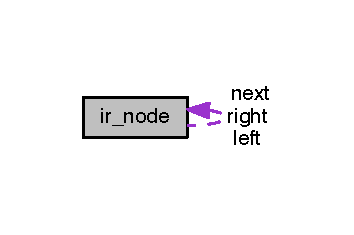
\includegraphics[width=170pt]{structir__node__coll__graph}
\end{center}
\end{figure}
\subsection*{Data Fields}
\begin{DoxyCompactItemize}
\item 
struct \hyperlink{structir__node}{ir\+\_\+node} $\ast$ \hyperlink{structir__node_ab6ecf53bf92c825b620435fc93a6b6ee}{left}
\item 
struct \hyperlink{structir__node}{ir\+\_\+node} $\ast$ \hyperlink{structir__node_ab1d37e8ddfafb50b2633b66af37fb064}{next}
\item 
unsigned short int \hyperlink{structir__node_a4d977601c157f732bd7655d7a47e8545}{op}
\item 
struct \hyperlink{structir__node}{ir\+\_\+node} $\ast$ \hyperlink{structir__node_ab72283b06a90004232c315bc52b0e9b5}{right}
\item 
int \hyperlink{structir__node_a4cd43e9ea9717dc8bda34aa8ca5f8d35}{value}
\end{DoxyCompactItemize}


\subsection{Detailed Description}
node of the intermediate representation parse tree 

Node of the intermediate representation parse tree 

Definition at line 101 of file roll.\+h.



\subsection{Field Documentation}
\hypertarget{structir__node_ab6ecf53bf92c825b620435fc93a6b6ee}{}\index{ir\+\_\+node@{ir\+\_\+node}!left@{left}}
\index{left@{left}!ir\+\_\+node@{ir\+\_\+node}}
\subsubsection[{left}]{\setlength{\rightskip}{0pt plus 5cm}struct {\bf ir\+\_\+node}$\ast$ ir\+\_\+node\+::left}\label{structir__node_ab6ecf53bf92c825b620435fc93a6b6ee}
Left branch 

Definition at line 102 of file roll.\+h.



Referenced by allocate\+\_\+node(), new\+\_\+op(), and roll\+\_\+expression().

\hypertarget{structir__node_ab1d37e8ddfafb50b2633b66af37fb064}{}\index{ir\+\_\+node@{ir\+\_\+node}!next@{next}}
\index{next@{next}!ir\+\_\+node@{ir\+\_\+node}}
\subsubsection[{next}]{\setlength{\rightskip}{0pt plus 5cm}struct {\bf ir\+\_\+node}$\ast$ ir\+\_\+node\+::next}\label{structir__node_ab1d37e8ddfafb50b2633b66af37fb064}
Next tree 

Definition at line 104 of file roll.\+h.



Referenced by allocate\+\_\+node(), and roll\+\_\+expression().

\hypertarget{structir__node_a4d977601c157f732bd7655d7a47e8545}{}\index{ir\+\_\+node@{ir\+\_\+node}!op@{op}}
\index{op@{op}!ir\+\_\+node@{ir\+\_\+node}}
\subsubsection[{op}]{\setlength{\rightskip}{0pt plus 5cm}unsigned short int ir\+\_\+node\+::op}\label{structir__node_a4d977601c157f732bd7655d7a47e8545}
Node type 

Definition at line 105 of file roll.\+h.



Referenced by allocate\+\_\+node(), new\+\_\+dice(), new\+\_\+number(), new\+\_\+op(), and roll\+\_\+expression().

\hypertarget{structir__node_ab72283b06a90004232c315bc52b0e9b5}{}\index{ir\+\_\+node@{ir\+\_\+node}!right@{right}}
\index{right@{right}!ir\+\_\+node@{ir\+\_\+node}}
\subsubsection[{right}]{\setlength{\rightskip}{0pt plus 5cm}struct {\bf ir\+\_\+node}$\ast$ ir\+\_\+node\+::right}\label{structir__node_ab72283b06a90004232c315bc52b0e9b5}
Right branch 

Definition at line 103 of file roll.\+h.



Referenced by allocate\+\_\+node(), new\+\_\+dice(), new\+\_\+op(), and roll\+\_\+expression().

\hypertarget{structir__node_a4cd43e9ea9717dc8bda34aa8ca5f8d35}{}\index{ir\+\_\+node@{ir\+\_\+node}!value@{value}}
\index{value@{value}!ir\+\_\+node@{ir\+\_\+node}}
\subsubsection[{value}]{\setlength{\rightskip}{0pt plus 5cm}int ir\+\_\+node\+::value}\label{structir__node_a4cd43e9ea9717dc8bda34aa8ca5f8d35}
Optional node value 

Definition at line 106 of file roll.\+h.



Referenced by allocate\+\_\+node(), new\+\_\+dice(), new\+\_\+number(), new\+\_\+op(), and roll\+\_\+expression().



The documentation for this struct was generated from the following file\+:\begin{DoxyCompactItemize}
\item 
\hyperlink{roll_8h}{roll.\+h}\end{DoxyCompactItemize}

\chapter{File Documentation}
\hypertarget{roll_8c}{}\section{roll.\+c File Reference}
\label{roll_8c}\index{roll.\+c@{roll.\+c}}


The main application file.  


{\ttfamily \#include \char`\"{}roll.\+h\char`\"{}}\\*
Include dependency graph for roll.\+c\+:
\nopagebreak
\begin{figure}[H]
\begin{center}
\leavevmode
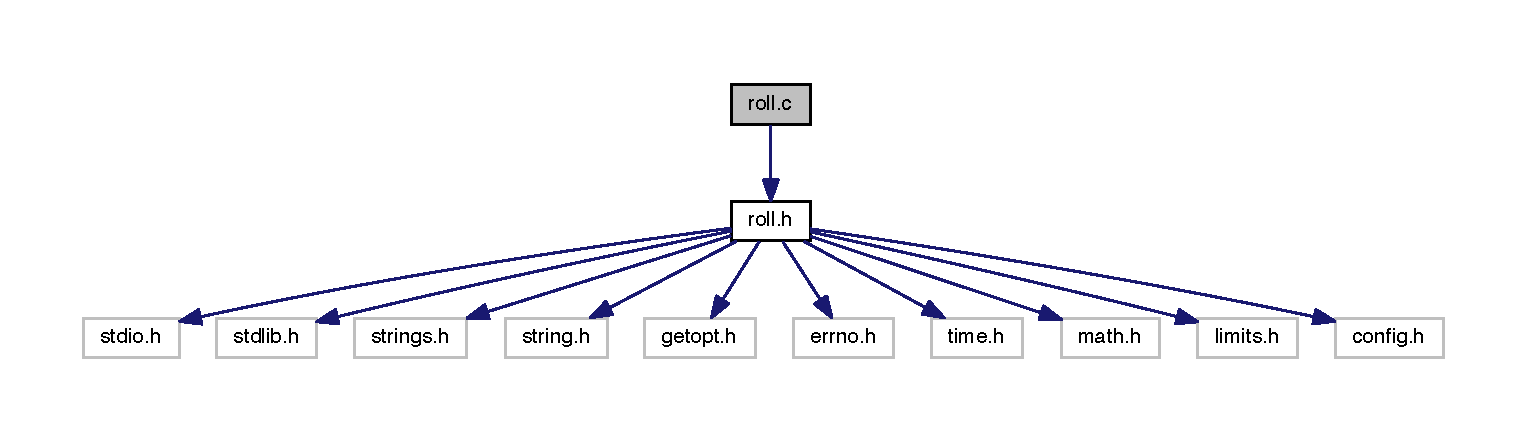
\includegraphics[width=350pt]{roll_8c__incl}
\end{center}
\end{figure}
\subsection*{Functions}
\begin{DoxyCompactItemize}
\item 
struct \hyperlink{structir__node}{ir\+\_\+node} $\ast$ \hyperlink{roll_8c_ab19c6534375437b3fa360f51198028f5}{allocate\+\_\+node} (void)
\begin{DoxyCompactList}\small\item\em Allocates a new I\+R node. \end{DoxyCompactList}\item 
int \hyperlink{roll_8c_aa9f19e181fbf7ceeb8e9cad996d29ef9}{compare} (const void $\ast$p1, const void $\ast$p2)
\begin{DoxyCompactList}\small\item\em Comparison function for qsort. \end{DoxyCompactList}\item 
void \hyperlink{roll_8c_a8e1bf3d5ea0a885f81e71d2023a55777}{error} (char $\ast$message)
\begin{DoxyCompactList}\small\item\em Prints the specified error message and exits with a failure status. \end{DoxyCompactList}\item 
int \hyperlink{roll_8c_a3c04138a5bfe5d72780bb7e82a18e627}{main} (int argc, char $\ast$$\ast$argv)
\begin{DoxyCompactList}\small\item\em Main program. \end{DoxyCompactList}\item 
struct \hyperlink{structir__node}{ir\+\_\+node} $\ast$ \hyperlink{roll_8c_aa255c368423347571a5a7ec8a01840cd}{new\+\_\+dice} (struct \hyperlink{structir__node}{ir\+\_\+node} $\ast$sides)
\begin{DoxyCompactList}\small\item\em Allocates a new D\+I\+C\+E node. \end{DoxyCompactList}\item 
struct \hyperlink{structir__node}{ir\+\_\+node} $\ast$ \hyperlink{roll_8c_a9708fd7a304b37bac39a25b0a8fe889e}{new\+\_\+number} (int number)
\begin{DoxyCompactList}\small\item\em Allocates a new N\+U\+M\+B\+E\+R node. \end{DoxyCompactList}\item 
struct \hyperlink{structir__node}{ir\+\_\+node} $\ast$ \hyperlink{roll_8c_ad29ccfc41dabb89e317de25329c3d279}{new\+\_\+op} (unsigned short int op, struct \hyperlink{structir__node}{ir\+\_\+node} $\ast$left, struct \hyperlink{structir__node}{ir\+\_\+node} $\ast$right)
\begin{DoxyCompactList}\small\item\em Allocates a new O\+P node. \end{DoxyCompactList}\item 
int \hyperlink{roll_8c_a25887d1873a9df6c717c4daae7d4efc2}{roll} (int dice)
\begin{DoxyCompactList}\small\item\em Rolls an n-\/sided dice. \end{DoxyCompactList}\item 
int \hyperlink{roll_8c_a2526cf02acc7939c8a3c21264dddac50}{roll\+\_\+dice} (int sides)
\begin{DoxyCompactList}\small\item\em Wrapper for \hyperlink{roll_8c_a25887d1873a9df6c717c4daae7d4efc2}{roll(int dice)} translates special dices (e.\+g., d\%) \end{DoxyCompactList}\item 
int \hyperlink{roll_8c_ad4c76f688ad79c99d3c39f54358964c8}{roll\+\_\+expression} (struct \hyperlink{structir__node}{ir\+\_\+node} $\ast$node, int print)
\begin{DoxyCompactList}\small\item\em Roll dices and compute expressions. \end{DoxyCompactList}\item 
\hypertarget{roll_8c_a2ef30c42cbc289d899a8be5d2d8f77d0}{}void \hyperlink{roll_8c_a2ef30c42cbc289d899a8be5d2d8f77d0}{usage} ()\label{roll_8c_a2ef30c42cbc289d899a8be5d2d8f77d0}

\begin{DoxyCompactList}\small\item\em Prints the program\textquotesingle{}s usage. \end{DoxyCompactList}\end{DoxyCompactItemize}
\subsection*{Variables}
\begin{DoxyCompactItemize}
\item 
int \hyperlink{roll_8c_ab1b14e1b3006d5f4665e1f5a74e25f93}{positive\+\_\+flag}
\item 
int \hyperlink{roll_8c_abec29e6443957b8a01502b04f2e9ba39}{sum\+\_\+flag} = \hyperlink{roll_8h_aa93f0eb578d23995850d61f7d61c55c1}{F\+A\+L\+S\+E}
\item 
static int \hyperlink{roll_8c_a4c7699f4d1b8ee152b8d35bbc579430b}{verbose\+\_\+flag} = \hyperlink{roll_8h_aa93f0eb578d23995850d61f7d61c55c1}{F\+A\+L\+S\+E}
\item 
static int \hyperlink{roll_8c_a541cb25faf92a00e9ecaa761baed4c2f}{version\+\_\+flag} = \hyperlink{roll_8h_aa93f0eb578d23995850d61f7d61c55c1}{F\+A\+L\+S\+E}
\end{DoxyCompactItemize}


\subsection{Detailed Description}
The main application file. 

\begin{DoxyAuthor}{Author}
Matteo Corti 
\end{DoxyAuthor}


\subsection{Function Documentation}
\hypertarget{roll_8c_ab19c6534375437b3fa360f51198028f5}{}\index{roll.\+c@{roll.\+c}!allocate\+\_\+node@{allocate\+\_\+node}}
\index{allocate\+\_\+node@{allocate\+\_\+node}!roll.\+c@{roll.\+c}}
\subsubsection[{allocate\+\_\+node(void)}]{\setlength{\rightskip}{0pt plus 5cm}struct {\bf ir\+\_\+node}$\ast$ allocate\+\_\+node (
\begin{DoxyParamCaption}
\item[{void}]{}
\end{DoxyParamCaption}
)}\label{roll_8c_ab19c6534375437b3fa360f51198028f5}


Allocates a new I\+R node. 

\begin{DoxyReturn}{Returns}
Newly allocated node 
\end{DoxyReturn}


Definition at line 266 of file roll.\+c.



References error(), ir\+\_\+node\+::left, ir\+\_\+node\+::next, ir\+\_\+node\+::op, ir\+\_\+node\+::right, and ir\+\_\+node\+::value.



Referenced by new\+\_\+dice(), new\+\_\+number(), and new\+\_\+op().


\begin{DoxyCode}
266                                          \{
267 
268   \textcolor{keyword}{struct }\hyperlink{structir__node}{ir\_node} * node = malloc(\textcolor{keyword}{sizeof}(\textcolor{keyword}{struct} \hyperlink{structir__node}{ir\_node}));
269   \textcolor{keywordflow}{if} (node == NULL) \{
270     \hyperlink{roll_8c_a8e1bf3d5ea0a885f81e71d2023a55777}{error}(\textcolor{stringliteral}{"Out of memory\(\backslash\)n"});
271     exit(EXIT\_FAILURE);
272   \}
273 
274   \textcolor{comment}{/* initialize default values */}
275   node->\hyperlink{structir__node_ab6ecf53bf92c825b620435fc93a6b6ee}{left}  = NULL;
276   node->\hyperlink{structir__node_ab72283b06a90004232c315bc52b0e9b5}{right} = NULL;
277   node->\hyperlink{structir__node_ab1d37e8ddfafb50b2633b66af37fb064}{next}  = NULL;
278   node->\hyperlink{structir__node_a4d977601c157f732bd7655d7a47e8545}{op}    = 0;
279   node->\hyperlink{structir__node_a4cd43e9ea9717dc8bda34aa8ca5f8d35}{value} = 0;
280   
281   \textcolor{keywordflow}{return} node;
282   
283 \}
\end{DoxyCode}


Here is the call graph for this function\+:
\nopagebreak
\begin{figure}[H]
\begin{center}
\leavevmode
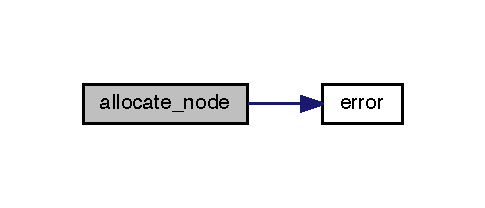
\includegraphics[width=233pt]{roll_8c_ab19c6534375437b3fa360f51198028f5_cgraph}
\end{center}
\end{figure}


\hypertarget{roll_8c_aa9f19e181fbf7ceeb8e9cad996d29ef9}{}\index{roll.\+c@{roll.\+c}!compare@{compare}}
\index{compare@{compare}!roll.\+c@{roll.\+c}}
\subsubsection[{compare(const void $\ast$p1, const void $\ast$p2)}]{\setlength{\rightskip}{0pt plus 5cm}int compare (
\begin{DoxyParamCaption}
\item[{const void $\ast$}]{p1, }
\item[{const void $\ast$}]{p2}
\end{DoxyParamCaption}
)}\label{roll_8c_aa9f19e181fbf7ceeb8e9cad996d29ef9}


Comparison function for qsort. 


\begin{DoxyParams}{Parameters}
{\em } & \\
\hline
\end{DoxyParams}


Definition at line 306 of file roll.\+c.



Referenced by roll\+\_\+expression().


\begin{DoxyCode}
306                                               \{
307 
308   \textcolor{keyword}{const} \textcolor{keywordtype}{int} i1 = *((\textcolor{keyword}{const} \textcolor{keywordtype}{int} *)p1);
309   \textcolor{keyword}{const} \textcolor{keywordtype}{int} i2 = *((\textcolor{keyword}{const} \textcolor{keywordtype}{int} *)p2);
310 
311   \textcolor{keywordflow}{if} (i1 > i2) \{
312     \textcolor{keywordflow}{return} 1;
313   \} \textcolor{keywordflow}{else} \textcolor{keywordflow}{if} (i1 < i2) \{
314     \textcolor{keywordflow}{return} -1;
315   \} \textcolor{keywordflow}{else} \{
316     \textcolor{keywordflow}{return} 0;
317   \}
318   
319 \}
\end{DoxyCode}
\hypertarget{roll_8c_a8e1bf3d5ea0a885f81e71d2023a55777}{}\index{roll.\+c@{roll.\+c}!error@{error}}
\index{error@{error}!roll.\+c@{roll.\+c}}
\subsubsection[{error(char $\ast$message)}]{\setlength{\rightskip}{0pt plus 5cm}void error (
\begin{DoxyParamCaption}
\item[{char $\ast$}]{message}
\end{DoxyParamCaption}
)}\label{roll_8c_a8e1bf3d5ea0a885f81e71d2023a55777}


Prints the specified error message and exits with a failure status. 


\begin{DoxyParams}{Parameters}
{\em } & \\
\hline
\end{DoxyParams}


Definition at line 50 of file roll.\+c.



Referenced by allocate\+\_\+node(), main(), and roll\+\_\+expression().


\begin{DoxyCode}
50                            \{
51   fprintf(stderr, \textcolor{stringliteral}{"\(\backslash\)nError: %s\(\backslash\)n"}, message);
52   exit(EXIT\_FAILURE);
53 \}
\end{DoxyCode}
\hypertarget{roll_8c_a3c04138a5bfe5d72780bb7e82a18e627}{}\index{roll.\+c@{roll.\+c}!main@{main}}
\index{main@{main}!roll.\+c@{roll.\+c}}
\subsubsection[{main(int argc, char $\ast$$\ast$argv)}]{\setlength{\rightskip}{0pt plus 5cm}int main (
\begin{DoxyParamCaption}
\item[{int}]{argc, }
\item[{char $\ast$$\ast$}]{argv}
\end{DoxyParamCaption}
)}\label{roll_8c_a3c04138a5bfe5d72780bb7e82a18e627}


Main program. 


\begin{DoxyParams}{Parameters}
{\em } & \\
\hline
\end{DoxyParams}


Definition at line 150 of file roll.\+c.



References error(), E\+X\+P\+R\+E\+S\+S\+I\+O\+N\+\_\+\+S\+I\+Z\+E, positive\+\_\+flag, srandomdev, sum\+\_\+flag, T\+R\+U\+E, usage(), verbose\+\_\+flag, and version\+\_\+flag.


\begin{DoxyCode}
150                                 \{
151 
152   \textcolor{keywordtype}{char}   expression[\hyperlink{roll_8h_ae05abae0cdd75043c8e635c5c90f9272}{EXPRESSION\_SIZE}];
153   \textcolor{keywordtype}{int}    expression\_size;
154   
155   \hyperlink{roll_8h_af3bc8a5595302da2f2984141e633266f}{srandomdev}();
156      
157   \textcolor{keywordflow}{while} (\hyperlink{roll_8h_aa8cecfc5c5c054d2875c03e77b7be15d}{TRUE}) \{
158 
159     \textcolor{keyword}{static} \textcolor{keyword}{struct }option long\_options[] = \{
160       \{\textcolor{stringliteral}{"sum-series"},  no\_argument,       NULL, \textcolor{charliteral}{'s'}\},
161       \{\textcolor{stringliteral}{"positive"},    no\_argument,       NULL, \textcolor{charliteral}{'p'}\},
162       \{\textcolor{stringliteral}{"verbose"},     no\_argument,       NULL, \textcolor{charliteral}{'v'}\},
163       \{\textcolor{stringliteral}{"version"},     no\_argument,       &\hyperlink{roll_8c_a541cb25faf92a00e9ecaa761baed4c2f}{version\_flag}, \hyperlink{roll_8h_aa8cecfc5c5c054d2875c03e77b7be15d}{TRUE}\},
164       \{\textcolor{stringliteral}{"help"},        no\_argument,       NULL, \textcolor{charliteral}{'h'}\},
165 \textcolor{preprocessor}{#ifdef DEBUG}
166       \{\textcolor{stringliteral}{"debug"},       no\_argument,       NULL, \textcolor{charliteral}{'d'}\},
167 \textcolor{preprocessor}{#endif}
168       \{NULL, 0, NULL, 0\}
169     \};
170 
171     \textcolor{comment}{/* getopt\_long stores the option index here. */}
172     \textcolor{keywordtype}{int} option\_index = 0;
173 
174     \textcolor{keywordtype}{int} c;
175     
176 \textcolor{preprocessor}{#ifdef DEBUG}
177     c = getopt\_long (argc, argv, \textcolor{stringliteral}{"hvspd"},
178              long\_options, &option\_index);
179 \textcolor{preprocessor}{#else}
180     c = getopt\_long (argc, argv, \textcolor{stringliteral}{"hvsp"},
181              long\_options, &option\_index);
182 \textcolor{preprocessor}{#endif}
183     
184     \textcolor{comment}{/* Detect the end of the options. */}
185     \textcolor{keywordflow}{if} (c == -1)
186       \textcolor{keywordflow}{break};
187      
188     \textcolor{keywordflow}{switch} (c) \{
189 
190     \textcolor{keywordflow}{case} \textcolor{charliteral}{'v'}:
191       \hyperlink{roll_8c_a4c7699f4d1b8ee152b8d35bbc579430b}{verbose\_flag} = \hyperlink{roll_8h_aa8cecfc5c5c054d2875c03e77b7be15d}{TRUE};
192       \textcolor{keywordflow}{break};
193 
194     \textcolor{keywordflow}{case} \textcolor{charliteral}{'s'}:
195       \hyperlink{roll_8c_abec29e6443957b8a01502b04f2e9ba39}{sum\_flag} = \hyperlink{roll_8h_aa8cecfc5c5c054d2875c03e77b7be15d}{TRUE};
196       \textcolor{keywordflow}{break};
197       
198     \textcolor{keywordflow}{case} \textcolor{charliteral}{'p'}:
199       \hyperlink{roll_8c_ab1b14e1b3006d5f4665e1f5a74e25f93}{positive\_flag} = \hyperlink{roll_8h_aa8cecfc5c5c054d2875c03e77b7be15d}{TRUE};
200       \textcolor{keywordflow}{break};
201 
202     \textcolor{keywordflow}{case} \textcolor{charliteral}{'h'}:
203       \hyperlink{roll_8c_a2ef30c42cbc289d899a8be5d2d8f77d0}{usage}();
204       exit(0);
205 
206     \textcolor{keywordflow}{case} \textcolor{charliteral}{'?'}:
207       \hyperlink{roll_8c_a2ef30c42cbc289d899a8be5d2d8f77d0}{usage}();
208       \textcolor{comment}{/* getopt\_long already printed an error message. */}
209       exit(EXIT\_SUCCESS);
210 
211 \textcolor{preprocessor}{#ifdef DEBUG}
212     \textcolor{keywordflow}{case} \textcolor{charliteral}{'d'}:
213       debug\_flag++;
214       \textcolor{keywordflow}{break};      
215 \textcolor{preprocessor}{#endif}
216       
217     \textcolor{keywordflow}{case} 0:
218       \textcolor{keywordflow}{break};
219 
220     \textcolor{keywordflow}{default}:
221       abort ();
222     \}
223 
224   \}
225 
226   \textcolor{keywordflow}{if} (\hyperlink{roll_8c_a541cb25faf92a00e9ecaa761baed4c2f}{version\_flag}) \{
227     printf(\textcolor{stringliteral}{"%s %s\(\backslash\)n"}, PACKAGE\_NAME, PACKAGE\_VERSION);
228     exit(EXIT\_SUCCESS);
229   \}      
230 
231   argc -= optind;
232   argv += optind;         
233   
234   \textcolor{comment}{/* build string to parse */}
235   expression[0] = \textcolor{charliteral}{'\(\backslash\)0'};
236   expression\_size = 0;
237   \textcolor{keywordflow}{while}(argc>0) \{
238     expression\_size += strlen(*argv);
239     \textcolor{keywordflow}{if} (expression\_size >= \hyperlink{roll_8h_ae05abae0cdd75043c8e635c5c90f9272}{EXPRESSION\_SIZE}) \{
240       \hyperlink{roll_8c_a8e1bf3d5ea0a885f81e71d2023a55777}{error}(\textcolor{stringliteral}{"Expression too long!\(\backslash\)n"});
241     \}
242     strncat(expression, *argv, \hyperlink{roll_8h_ae05abae0cdd75043c8e635c5c90f9272}{EXPRESSION\_SIZE}-1);
243     argc--;
244     argv++;
245   \}
246   
247   \textcolor{keywordflow}{if} (expression\_size > 0) \{
248     
249     yy\_scan\_string(expression);
250 
251     yyparse();
252 
253   \} \textcolor{keywordflow}{else} \{
254     \hyperlink{roll_8c_a8e1bf3d5ea0a885f81e71d2023a55777}{error}(\textcolor{stringliteral}{"No expression provided!\(\backslash\)nPlease use the \(\backslash\)"-h\(\backslash\)" option.\(\backslash\)n"});
255     exit(EXIT\_FAILURE);
256   \}
257 
258   \textcolor{keywordflow}{return} 0;
259 
260 \}
\end{DoxyCode}


Here is the call graph for this function\+:
\nopagebreak
\begin{figure}[H]
\begin{center}
\leavevmode
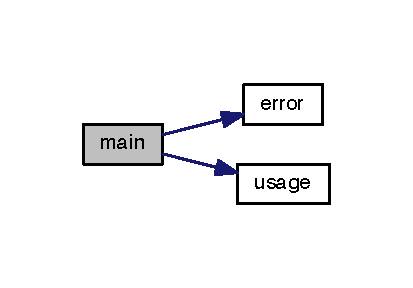
\includegraphics[width=198pt]{roll_8c_a3c04138a5bfe5d72780bb7e82a18e627_cgraph}
\end{center}
\end{figure}


\hypertarget{roll_8c_aa255c368423347571a5a7ec8a01840cd}{}\index{roll.\+c@{roll.\+c}!new\+\_\+dice@{new\+\_\+dice}}
\index{new\+\_\+dice@{new\+\_\+dice}!roll.\+c@{roll.\+c}}
\subsubsection[{new\+\_\+dice(struct ir\+\_\+node $\ast$sides)}]{\setlength{\rightskip}{0pt plus 5cm}struct {\bf ir\+\_\+node}$\ast$ new\+\_\+dice (
\begin{DoxyParamCaption}
\item[{struct {\bf ir\+\_\+node} $\ast$}]{sides}
\end{DoxyParamCaption}
)}\label{roll_8c_aa255c368423347571a5a7ec8a01840cd}


Allocates a new D\+I\+C\+E node. 


\begin{DoxyParams}{Parameters}
{\em } & \\
\hline
\end{DoxyParams}


Definition at line 344 of file roll.\+c.



References allocate\+\_\+node(), ir\+\_\+node\+::op, O\+P\+\_\+\+D\+I\+C\+E, ir\+\_\+node\+::right, and ir\+\_\+node\+::value.


\begin{DoxyCode}
344                                                     \{
345   
346   \textcolor{keyword}{struct }\hyperlink{structir__node}{ir\_node} * node = \hyperlink{roll_8c_ab19c6534375437b3fa360f51198028f5}{allocate\_node}();
347   node->\hyperlink{structir__node_a4d977601c157f732bd7655d7a47e8545}{op}    = \hyperlink{roll_8h_ac22133e25cbb119a03e18be7e2b029f4}{OP\_DICE};
348   node->\hyperlink{structir__node_a4cd43e9ea9717dc8bda34aa8ca5f8d35}{value} = 0;
349   node->\hyperlink{structir__node_ab72283b06a90004232c315bc52b0e9b5}{right} = sides;
350   \textcolor{keywordflow}{return} node;
351   
352 \}
\end{DoxyCode}


Here is the call graph for this function\+:
\nopagebreak
\begin{figure}[H]
\begin{center}
\leavevmode
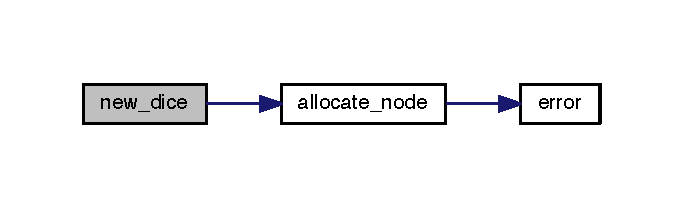
\includegraphics[width=328pt]{roll_8c_aa255c368423347571a5a7ec8a01840cd_cgraph}
\end{center}
\end{figure}


\hypertarget{roll_8c_a9708fd7a304b37bac39a25b0a8fe889e}{}\index{roll.\+c@{roll.\+c}!new\+\_\+number@{new\+\_\+number}}
\index{new\+\_\+number@{new\+\_\+number}!roll.\+c@{roll.\+c}}
\subsubsection[{new\+\_\+number(int number)}]{\setlength{\rightskip}{0pt plus 5cm}struct {\bf ir\+\_\+node}$\ast$ new\+\_\+number (
\begin{DoxyParamCaption}
\item[{int}]{number}
\end{DoxyParamCaption}
)}\label{roll_8c_a9708fd7a304b37bac39a25b0a8fe889e}


Allocates a new N\+U\+M\+B\+E\+R node. 


\begin{DoxyParams}{Parameters}
{\em } & \\
\hline
\end{DoxyParams}


Definition at line 290 of file roll.\+c.



References allocate\+\_\+node(), ir\+\_\+node\+::op, O\+P\+\_\+\+N\+U\+M\+B\+E\+R, and ir\+\_\+node\+::value.


\begin{DoxyCode}
290                                            \{
291 
292   \textcolor{keyword}{struct }\hyperlink{structir__node}{ir\_node} * node = \hyperlink{roll_8c_ab19c6534375437b3fa360f51198028f5}{allocate\_node}();
293   node->\hyperlink{structir__node_a4d977601c157f732bd7655d7a47e8545}{op}    = \hyperlink{roll_8h_aee5d81dd03df6e8030c9f559ec346f95}{OP\_NUMBER};
294   node->\hyperlink{structir__node_a4cd43e9ea9717dc8bda34aa8ca5f8d35}{value} = number;
295 
296   \textcolor{keywordflow}{return} node;
297 
298 \}
\end{DoxyCode}


Here is the call graph for this function\+:
\nopagebreak
\begin{figure}[H]
\begin{center}
\leavevmode
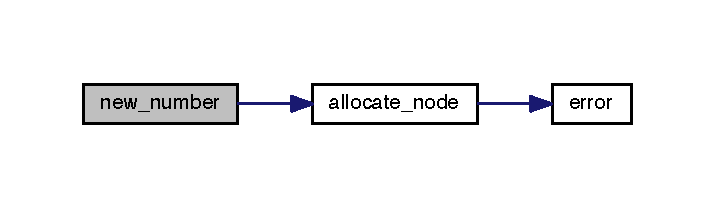
\includegraphics[width=343pt]{roll_8c_a9708fd7a304b37bac39a25b0a8fe889e_cgraph}
\end{center}
\end{figure}


\hypertarget{roll_8c_ad29ccfc41dabb89e317de25329c3d279}{}\index{roll.\+c@{roll.\+c}!new\+\_\+op@{new\+\_\+op}}
\index{new\+\_\+op@{new\+\_\+op}!roll.\+c@{roll.\+c}}
\subsubsection[{new\+\_\+op(unsigned short int op, struct ir\+\_\+node $\ast$left, struct ir\+\_\+node $\ast$right)}]{\setlength{\rightskip}{0pt plus 5cm}struct {\bf ir\+\_\+node}$\ast$ new\+\_\+op (
\begin{DoxyParamCaption}
\item[{unsigned short int}]{op, }
\item[{struct {\bf ir\+\_\+node} $\ast$}]{left, }
\item[{struct {\bf ir\+\_\+node} $\ast$}]{right}
\end{DoxyParamCaption}
)}\label{roll_8c_ad29ccfc41dabb89e317de25329c3d279}


Allocates a new O\+P node. 


\begin{DoxyParams}{Parameters}
{\em } & \\
\hline
\end{DoxyParams}


Definition at line 328 of file roll.\+c.



References allocate\+\_\+node(), ir\+\_\+node\+::left, ir\+\_\+node\+::op, ir\+\_\+node\+::right, and ir\+\_\+node\+::value.


\begin{DoxyCode}
328                                                                                                 \{
329 
330   \textcolor{keyword}{struct }\hyperlink{structir__node}{ir\_node} * node = \hyperlink{roll_8c_ab19c6534375437b3fa360f51198028f5}{allocate\_node}();
331   node->\hyperlink{structir__node_a4d977601c157f732bd7655d7a47e8545}{op}    = \hyperlink{structir__node_a4d977601c157f732bd7655d7a47e8545}{op};
332   node->\hyperlink{structir__node_a4cd43e9ea9717dc8bda34aa8ca5f8d35}{value} = 0;
333   node->\hyperlink{structir__node_ab6ecf53bf92c825b620435fc93a6b6ee}{left}  = \hyperlink{structir__node_ab6ecf53bf92c825b620435fc93a6b6ee}{left};
334   node->\hyperlink{structir__node_ab72283b06a90004232c315bc52b0e9b5}{right} = \hyperlink{structir__node_ab72283b06a90004232c315bc52b0e9b5}{right};
335   \textcolor{keywordflow}{return} node;
336   
337 \}
\end{DoxyCode}


Here is the call graph for this function\+:
\nopagebreak
\begin{figure}[H]
\begin{center}
\leavevmode
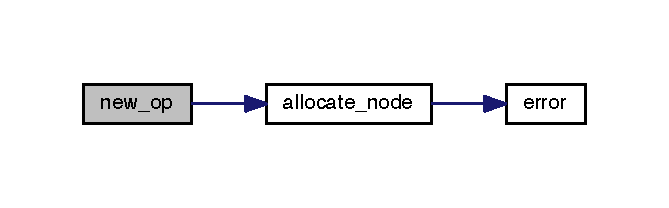
\includegraphics[width=321pt]{roll_8c_ad29ccfc41dabb89e317de25329c3d279_cgraph}
\end{center}
\end{figure}


\hypertarget{roll_8c_a25887d1873a9df6c717c4daae7d4efc2}{}\index{roll.\+c@{roll.\+c}!roll@{roll}}
\index{roll@{roll}!roll.\+c@{roll.\+c}}
\subsubsection[{roll(int dice)}]{\setlength{\rightskip}{0pt plus 5cm}int roll (
\begin{DoxyParamCaption}
\item[{int}]{dice}
\end{DoxyParamCaption}
)}\label{roll_8c_a25887d1873a9df6c717c4daae7d4efc2}


Rolls an n-\/sided dice. 


\begin{DoxyParams}{Parameters}
{\em } & \\
\hline
\end{DoxyParams}


Definition at line 124 of file roll.\+c.



Referenced by roll\+\_\+dice().


\begin{DoxyCode}
124                    \{
125 
126   \textcolor{comment}{/* }
127 \textcolor{comment}{   * In: W. H. Press et al,Numerical Recipes in C: The Art of}
128 \textcolor{comment}{   * Scientific Computing.  New York, Cambridge University Press,}
129 \textcolor{comment}{   * 1992, 2nd ed., p. 277}
130 \textcolor{comment}{   *}
131 \textcolor{comment}{   * "If you want to generate a random integer between 1 }
132 \textcolor{comment}{   *  and 10, you should always do it by using high-order}
133 \textcolor{comment}{   *  bits, as in}
134 \textcolor{comment}{   *}
135 \textcolor{comment}{   *  j=1+(int) (10.0*rand()/(RAND\_MAX+1.0));}
136 \textcolor{comment}{   */}
137 
138   \textcolor{keywordtype}{int} res = 1+(int)(((\textcolor{keywordtype}{double})dice)*random()/(RAND\_MAX+1.0));
139 
140   \textcolor{keywordflow}{return} res;
141 
142 \}
\end{DoxyCode}
\hypertarget{roll_8c_a2526cf02acc7939c8a3c21264dddac50}{}\index{roll.\+c@{roll.\+c}!roll\+\_\+dice@{roll\+\_\+dice}}
\index{roll\+\_\+dice@{roll\+\_\+dice}!roll.\+c@{roll.\+c}}
\subsubsection[{roll\+\_\+dice(int sides)}]{\setlength{\rightskip}{0pt plus 5cm}int roll\+\_\+dice (
\begin{DoxyParamCaption}
\item[{int}]{sides}
\end{DoxyParamCaption}
)}\label{roll_8c_a2526cf02acc7939c8a3c21264dddac50}


Wrapper for \hyperlink{roll_8c_a25887d1873a9df6c717c4daae7d4efc2}{roll(int dice)} translates special dices (e.\+g., d\%) 


\begin{DoxyParams}{Parameters}
{\em } & \\
\hline
\end{DoxyParams}


Definition at line 59 of file roll.\+c.



References H\+U\+N\+D\+R\+E\+D, roll(), and verbose\+\_\+flag.



Referenced by roll\+\_\+expression().


\begin{DoxyCode}
59                          \{
60 
61   \textcolor{keywordtype}{int} result = 0;
62   
63   \textcolor{keywordflow}{if} ( sides == \hyperlink{roll_8h_a625dac461fbab83b1c1d04f3aceeb8f3}{HUNDRED} ) \{
64     
65     \textcolor{comment}{/* d100 -> d10*10+d10 */}
66     
67     \textcolor{keywordtype}{int} d10 = \hyperlink{roll_8c_a25887d1873a9df6c717c4daae7d4efc2}{roll}(10);
68     \textcolor{keywordflow}{if} (\hyperlink{roll_8c_a4c7699f4d1b8ee152b8d35bbc579430b}{verbose\_flag}) \{
69       printf(\textcolor{stringliteral}{"d10 -> %i\(\backslash\)n"}, d10);
70     \}
71     d10 = d10 % 10;
72     
73     \textcolor{keywordtype}{int} d1 = \hyperlink{roll_8c_a25887d1873a9df6c717c4daae7d4efc2}{roll}(10);
74     \textcolor{keywordflow}{if} (\hyperlink{roll_8c_a4c7699f4d1b8ee152b8d35bbc579430b}{verbose\_flag}) \{
75       printf(\textcolor{stringliteral}{"d10 -> %i\(\backslash\)n"}, d1);
76     \}
77     
78     \textcolor{keywordflow}{if} (d1 == 0 && d10 == 0) \{
79       result = 100;
80     \} \textcolor{keywordflow}{else} \textcolor{keywordflow}{if} (d10 == 0) \{
81       result = d1;
82     \} \textcolor{keywordflow}{else} \{
83       result = d10*10 + d1;
84     \}
85 
86   \} \textcolor{keywordflow}{else} \textcolor{keywordflow}{if} ( sides == FUDGE\_DICE ) \{
87 
88     result = \hyperlink{roll_8c_a25887d1873a9df6c717c4daae7d4efc2}{roll}(3) - 2;
89 
90     \textcolor{keywordflow}{if} (\hyperlink{roll_8c_a4c7699f4d1b8ee152b8d35bbc579430b}{verbose\_flag}) \{
91 
92       \textcolor{keywordflow}{switch} (result) \{
93       \textcolor{keywordflow}{case} -1:
94         printf(\textcolor{stringliteral}{"dF -> -\(\backslash\)n"});
95         \textcolor{keywordflow}{break};
96       \textcolor{keywordflow}{case} 0:
97         printf(\textcolor{stringliteral}{"dF -> o\(\backslash\)n"});
98         \textcolor{keywordflow}{break};
99       \textcolor{keywordflow}{case} 1:
100         printf(\textcolor{stringliteral}{"dF -> +\(\backslash\)n"});
101         \textcolor{keywordflow}{break};        
102       \}
103     \}
104     
105   \} \textcolor{keywordflow}{else} \{
106 
107     result = \hyperlink{roll_8c_a25887d1873a9df6c717c4daae7d4efc2}{roll}(sides);
108     
109     \textcolor{keywordflow}{if} (\hyperlink{roll_8c_a4c7699f4d1b8ee152b8d35bbc579430b}{verbose\_flag}) \{
110       printf(\textcolor{stringliteral}{"d%i -> %i\(\backslash\)n"}, sides, result);
111     \}
112 
113   \}
114 
115   \textcolor{keywordflow}{return} result;
116   
117 \}
\end{DoxyCode}


Here is the call graph for this function\+:
\nopagebreak
\begin{figure}[H]
\begin{center}
\leavevmode
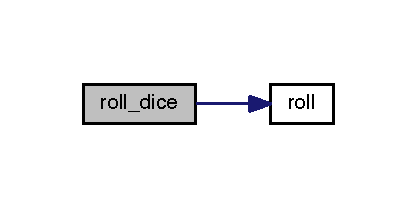
\includegraphics[width=200pt]{roll_8c_a2526cf02acc7939c8a3c21264dddac50_cgraph}
\end{center}
\end{figure}


\hypertarget{roll_8c_ad4c76f688ad79c99d3c39f54358964c8}{}\index{roll.\+c@{roll.\+c}!roll\+\_\+expression@{roll\+\_\+expression}}
\index{roll\+\_\+expression@{roll\+\_\+expression}!roll.\+c@{roll.\+c}}
\subsubsection[{roll\+\_\+expression(struct ir\+\_\+node $\ast$node, int print)}]{\setlength{\rightskip}{0pt plus 5cm}int roll\+\_\+expression (
\begin{DoxyParamCaption}
\item[{struct {\bf ir\+\_\+node} $\ast$}]{node, }
\item[{int}]{print}
\end{DoxyParamCaption}
)}\label{roll_8c_ad4c76f688ad79c99d3c39f54358964c8}


Roll dices and compute expressions. 


\begin{DoxyParams}{Parameters}
{\em } & \\
\hline
\end{DoxyParams}


Definition at line 376 of file roll.\+c.



References compare(), error(), F\+A\+L\+S\+E, ir\+\_\+node\+::left, ir\+\_\+node\+::next, ir\+\_\+node\+::op, O\+P\+\_\+\+D\+I\+C\+E, O\+P\+\_\+\+D\+I\+V, O\+P\+\_\+\+G\+E, O\+P\+\_\+\+G\+T, O\+P\+\_\+\+H\+I\+G\+H, O\+P\+\_\+\+L\+E, O\+P\+\_\+\+L\+O\+W, O\+P\+\_\+\+L\+T, O\+P\+\_\+\+M\+I\+N\+U\+S, O\+P\+\_\+\+N\+E, O\+P\+\_\+\+N\+U\+M\+B\+E\+R, O\+P\+\_\+\+P\+L\+U\+S, O\+P\+\_\+\+R\+E\+P, O\+P\+\_\+\+T\+I\+M\+E\+S, ir\+\_\+node\+::right, roll\+\_\+dice(), roll\+\_\+expression(), T\+R\+U\+E, and ir\+\_\+node\+::value.



Referenced by roll\+\_\+expression().


\begin{DoxyCode}
376                                                          \{
377 
378   \textcolor{keywordtype}{int}  high;
379   \textcolor{keywordtype}{int}  i;
380   \textcolor{keywordtype}{int}  limit;
381   \textcolor{keywordtype}{int}  low;
382   \textcolor{keywordtype}{int}  repetitions;
383   \textcolor{keywordtype}{int}  return\_value = 0;
384   \textcolor{keywordtype}{int}  sides;
385   \textcolor{keywordtype}{int}  tmp;
386   \textcolor{keywordtype}{int} * results;
387 
388   \textcolor{keyword}{struct }\hyperlink{structir__node}{ir\_node} * cur;
389 
390   cur = node;
391   \textcolor{keywordflow}{while} (cur != NULL) \{
392 
393     \textcolor{keywordtype}{int} sum = 0;
394 
395     \textcolor{keywordflow}{switch} (cur->\hyperlink{structir__node_a4d977601c157f732bd7655d7a47e8545}{op}) \{
396     
397     \textcolor{keywordflow}{case} \hyperlink{roll_8h_aee5d81dd03df6e8030c9f559ec346f95}{OP\_NUMBER}:
398       sum = cur->\hyperlink{structir__node_a4cd43e9ea9717dc8bda34aa8ca5f8d35}{value};
399       \textcolor{keywordflow}{break};
400 
401     \textcolor{keywordflow}{case} \hyperlink{roll_8h_abb555c8b38c708a0dd1c0a51849ce240}{OP\_REP}:
402 
403       \textcolor{keywordflow}{for} (i = 0; i < \hyperlink{roll_8c_ad4c76f688ad79c99d3c39f54358964c8}{roll\_expression}(cur->\hyperlink{structir__node_ab6ecf53bf92c825b620435fc93a6b6ee}{left}, \hyperlink{roll_8h_aa93f0eb578d23995850d61f7d61c55c1}{FALSE}); i++) \{
404         sum = checked\_sum( sum, \hyperlink{roll_8c_ad4c76f688ad79c99d3c39f54358964c8}{roll\_expression}(cur->\hyperlink{structir__node_ab72283b06a90004232c315bc52b0e9b5}{right}, 
      \hyperlink{roll_8h_aa93f0eb578d23995850d61f7d61c55c1}{FALSE}) );
405       \}
406       \textcolor{keywordflow}{break};
407       
408     \textcolor{keywordflow}{case} \hyperlink{roll_8h_ac22133e25cbb119a03e18be7e2b029f4}{OP\_DICE}:
409       sum = \hyperlink{roll_8c_a2526cf02acc7939c8a3c21264dddac50}{roll\_dice}( \hyperlink{roll_8c_ad4c76f688ad79c99d3c39f54358964c8}{roll\_expression}(cur->\hyperlink{structir__node_ab72283b06a90004232c315bc52b0e9b5}{right}, 
      \hyperlink{roll_8h_aa93f0eb578d23995850d61f7d61c55c1}{FALSE}) );
410       \textcolor{keywordflow}{break};
411       
412     \textcolor{keywordflow}{case} \hyperlink{roll_8h_a75a9903938da31e530a136d37a839848}{OP\_PLUS}:
413       sum = checked\_sum( \hyperlink{roll_8c_ad4c76f688ad79c99d3c39f54358964c8}{roll\_expression}( cur->\hyperlink{structir__node_ab6ecf53bf92c825b620435fc93a6b6ee}{left},  \hyperlink{roll_8h_aa93f0eb578d23995850d61f7d61c55c1}{FALSE} ),
414                          \hyperlink{roll_8c_ad4c76f688ad79c99d3c39f54358964c8}{roll\_expression}( cur->\hyperlink{structir__node_ab72283b06a90004232c315bc52b0e9b5}{right}, \hyperlink{roll_8h_aa93f0eb578d23995850d61f7d61c55c1}{FALSE} ) );
415       \textcolor{keywordflow}{break};
416       
417     \textcolor{keywordflow}{case} \hyperlink{roll_8h_ab62390fc8d7f39a0edfd26f5c30df780}{OP\_MINUS}:
418       sum = checked\_sum( \hyperlink{roll_8c_ad4c76f688ad79c99d3c39f54358964c8}{roll\_expression}( cur->\hyperlink{structir__node_ab6ecf53bf92c825b620435fc93a6b6ee}{left},  \hyperlink{roll_8h_aa93f0eb578d23995850d61f7d61c55c1}{FALSE} ),
419                          -\hyperlink{roll_8c_ad4c76f688ad79c99d3c39f54358964c8}{roll\_expression}( cur->\hyperlink{structir__node_ab72283b06a90004232c315bc52b0e9b5}{right}, \hyperlink{roll_8h_aa93f0eb578d23995850d61f7d61c55c1}{FALSE} ) );
420       \textcolor{keywordflow}{break};
421       
422     \textcolor{keywordflow}{case} \hyperlink{roll_8h_ac574cdf3dd634e54040f68400ec26e48}{OP\_TIMES}:
423       sum = checked\_multiplication( \hyperlink{roll_8c_ad4c76f688ad79c99d3c39f54358964c8}{roll\_expression}( cur->\hyperlink{structir__node_ab6ecf53bf92c825b620435fc93a6b6ee}{left},  
      \hyperlink{roll_8h_aa93f0eb578d23995850d61f7d61c55c1}{FALSE} ),
424                                    \hyperlink{roll_8c_ad4c76f688ad79c99d3c39f54358964c8}{roll\_expression}( cur->\hyperlink{structir__node_ab72283b06a90004232c315bc52b0e9b5}{right}, 
      \hyperlink{roll_8h_aa93f0eb578d23995850d61f7d61c55c1}{FALSE} ) );
425       \textcolor{keywordflow}{break};
426       
427     \textcolor{keywordflow}{case} \hyperlink{roll_8h_addec4be73478fb9243f0ea0087366641}{OP\_DIV}:
428       sum = (int)
429         ceil( (\textcolor{keywordtype}{float})\hyperlink{roll_8c_ad4c76f688ad79c99d3c39f54358964c8}{roll\_expression}( cur->\hyperlink{structir__node_ab6ecf53bf92c825b620435fc93a6b6ee}{left},  \hyperlink{roll_8h_aa93f0eb578d23995850d61f7d61c55c1}{FALSE} ) /
430               \hyperlink{roll_8c_ad4c76f688ad79c99d3c39f54358964c8}{roll\_expression}( cur->\hyperlink{structir__node_ab72283b06a90004232c315bc52b0e9b5}{right}, \hyperlink{roll_8h_aa93f0eb578d23995850d61f7d61c55c1}{FALSE} ) );
431       \textcolor{keywordflow}{break};
432       
433     \textcolor{keywordflow}{case} \hyperlink{roll_8h_ab9cc57ec763eabfbcdc422bcd574d50b}{OP\_HIGH}:
434 
435       sides       = \hyperlink{roll_8c_ad4c76f688ad79c99d3c39f54358964c8}{roll\_expression}(cur->\hyperlink{structir__node_ab72283b06a90004232c315bc52b0e9b5}{right}->\hyperlink{structir__node_ab72283b06a90004232c315bc52b0e9b5}{right}->
      \hyperlink{structir__node_ab72283b06a90004232c315bc52b0e9b5}{right}, \hyperlink{roll_8h_aa93f0eb578d23995850d61f7d61c55c1}{FALSE});
436       repetitions = \hyperlink{roll_8c_ad4c76f688ad79c99d3c39f54358964c8}{roll\_expression}(cur->\hyperlink{structir__node_ab72283b06a90004232c315bc52b0e9b5}{right}->\hyperlink{structir__node_ab6ecf53bf92c825b620435fc93a6b6ee}{left},  
      \hyperlink{roll_8h_aa93f0eb578d23995850d61f7d61c55c1}{FALSE});
437       high        = \hyperlink{roll_8c_ad4c76f688ad79c99d3c39f54358964c8}{roll\_expression}(cur->\hyperlink{structir__node_ab6ecf53bf92c825b620435fc93a6b6ee}{left}, \hyperlink{roll_8h_aa93f0eb578d23995850d61f7d61c55c1}{FALSE});      
438 
439       \textcolor{comment}{/* array to store the results to sort */}
440       \textcolor{keywordflow}{if} (!(results = malloc(\textcolor{keyword}{sizeof}(\textcolor{keywordtype}{int})*repetitions))) \{
441         \hyperlink{roll_8c_a8e1bf3d5ea0a885f81e71d2023a55777}{error}(\textcolor{stringliteral}{"Out of memory"});
442       \}
443       
444       \textcolor{keywordflow}{for}(i=0; i<repetitions; i++) \{
445         results[i] = \hyperlink{roll_8c_a2526cf02acc7939c8a3c21264dddac50}{roll\_dice}(sides);
446       \}
447       qsort(results, repetitions, \textcolor{keyword}{sizeof}(\textcolor{keywordtype}{int}), &\hyperlink{roll_8c_aa9f19e181fbf7ceeb8e9cad996d29ef9}{compare});
448 
449       \textcolor{keywordflow}{for}(i=(repetitions-high); i<repetitions; i++) \{
450         sum = checked\_sum( sum, results[i] );
451       \}
452       
453       free(results);
454       
455       \textcolor{keywordflow}{break};
456       
457     \textcolor{keywordflow}{case} \hyperlink{roll_8h_a8db1c769c2173f00e38f457c2d6450c0}{OP\_LOW}:
458       
459       sides       = \hyperlink{roll_8c_ad4c76f688ad79c99d3c39f54358964c8}{roll\_expression}(cur->\hyperlink{structir__node_ab72283b06a90004232c315bc52b0e9b5}{right}->\hyperlink{structir__node_ab72283b06a90004232c315bc52b0e9b5}{right}->
      \hyperlink{structir__node_ab72283b06a90004232c315bc52b0e9b5}{right}, \hyperlink{roll_8h_aa93f0eb578d23995850d61f7d61c55c1}{FALSE});
460       repetitions = \hyperlink{roll_8c_ad4c76f688ad79c99d3c39f54358964c8}{roll\_expression}(cur->\hyperlink{structir__node_ab72283b06a90004232c315bc52b0e9b5}{right}->\hyperlink{structir__node_ab6ecf53bf92c825b620435fc93a6b6ee}{left},  
      \hyperlink{roll_8h_aa93f0eb578d23995850d61f7d61c55c1}{FALSE});
461       low         = \hyperlink{roll_8c_ad4c76f688ad79c99d3c39f54358964c8}{roll\_expression}(cur->\hyperlink{structir__node_ab6ecf53bf92c825b620435fc93a6b6ee}{left}, \hyperlink{roll_8h_aa93f0eb578d23995850d61f7d61c55c1}{FALSE});
462       
463       \textcolor{keywordflow}{if} (cur->\hyperlink{structir__node_ab72283b06a90004232c315bc52b0e9b5}{right}->\hyperlink{structir__node_ab6ecf53bf92c825b620435fc93a6b6ee}{left} != NULL) \{
464         repetitions = \hyperlink{roll_8c_ad4c76f688ad79c99d3c39f54358964c8}{roll\_expression}(cur->\hyperlink{structir__node_ab72283b06a90004232c315bc52b0e9b5}{right}->\hyperlink{structir__node_ab6ecf53bf92c825b620435fc93a6b6ee}{left}, 
      \hyperlink{roll_8h_aa93f0eb578d23995850d61f7d61c55c1}{FALSE});
465       \}
466                   
467       \textcolor{comment}{/* array to store the results to sort */}
468       \textcolor{keywordflow}{if} (!(results = malloc(\textcolor{keyword}{sizeof}(\textcolor{keywordtype}{int})*repetitions))) \{
469         \hyperlink{roll_8c_a8e1bf3d5ea0a885f81e71d2023a55777}{error}(\textcolor{stringliteral}{"Out of memory"});
470       \}
471       
472       \textcolor{keywordflow}{for}(i=0; i<repetitions; i++) \{
473         results[i] = \hyperlink{roll_8c_a2526cf02acc7939c8a3c21264dddac50}{roll\_dice}(sides);
474       \}
475       qsort(results, repetitions, \textcolor{keyword}{sizeof}(\textcolor{keywordtype}{int}), &\hyperlink{roll_8c_aa9f19e181fbf7ceeb8e9cad996d29ef9}{compare});
476       \textcolor{keywordflow}{for}(i=0; i<low; i++) \{
477         sum = checked\_sum( sum, results[i] );
478       \}
479       
480       free(results);
481       
482       \textcolor{keywordflow}{break};
483 
484     \textcolor{keywordflow}{case} \hyperlink{roll_8h_a0fa482032824fe178a5c8510a6b268e8}{OP\_GT}:
485       
486       limit = \hyperlink{roll_8c_ad4c76f688ad79c99d3c39f54358964c8}{roll\_expression}(cur->\hyperlink{structir__node_ab72283b06a90004232c315bc52b0e9b5}{right}, \hyperlink{roll_8h_aa93f0eb578d23995850d61f7d61c55c1}{FALSE});      
487       tmp   = \hyperlink{roll_8c_ad4c76f688ad79c99d3c39f54358964c8}{roll\_expression}(cur->\hyperlink{structir__node_ab6ecf53bf92c825b620435fc93a6b6ee}{left},  \hyperlink{roll_8h_aa93f0eb578d23995850d61f7d61c55c1}{FALSE});
488       \textcolor{keywordflow}{while} (tmp <= limit) \{
489         tmp = \hyperlink{roll_8c_ad4c76f688ad79c99d3c39f54358964c8}{roll\_expression}(cur->\hyperlink{structir__node_ab6ecf53bf92c825b620435fc93a6b6ee}{left}, \hyperlink{roll_8h_aa93f0eb578d23995850d61f7d61c55c1}{FALSE});
490       \}
491       sum = checked\_sum( sum, tmp );
492       
493       \textcolor{keywordflow}{break};
494       
495     \textcolor{keywordflow}{case} \hyperlink{roll_8h_a81d577022941aa88aac9f64eef8d7faf}{OP\_GE}:
496       
497       limit = \hyperlink{roll_8c_ad4c76f688ad79c99d3c39f54358964c8}{roll\_expression}(cur->\hyperlink{structir__node_ab72283b06a90004232c315bc52b0e9b5}{right}, \hyperlink{roll_8h_aa93f0eb578d23995850d61f7d61c55c1}{FALSE});      
498       tmp   = \hyperlink{roll_8c_ad4c76f688ad79c99d3c39f54358964c8}{roll\_expression}(cur->\hyperlink{structir__node_ab6ecf53bf92c825b620435fc93a6b6ee}{left},  \hyperlink{roll_8h_aa93f0eb578d23995850d61f7d61c55c1}{FALSE});
499       \textcolor{keywordflow}{while} (tmp < limit) \{
500         tmp = \hyperlink{roll_8c_ad4c76f688ad79c99d3c39f54358964c8}{roll\_expression}(cur->\hyperlink{structir__node_ab6ecf53bf92c825b620435fc93a6b6ee}{left}, \hyperlink{roll_8h_aa93f0eb578d23995850d61f7d61c55c1}{FALSE});
501       \}
502       sum = checked\_sum( sum, tmp );
503       
504       \textcolor{keywordflow}{break};
505       
506     \textcolor{keywordflow}{case} \hyperlink{roll_8h_a09b4bd252d4ef2d01ba2394ce89096eb}{OP\_LT}:
507       
508       limit = \hyperlink{roll_8c_ad4c76f688ad79c99d3c39f54358964c8}{roll\_expression}(cur->\hyperlink{structir__node_ab72283b06a90004232c315bc52b0e9b5}{right}, \hyperlink{roll_8h_aa93f0eb578d23995850d61f7d61c55c1}{FALSE});      
509       tmp   = \hyperlink{roll_8c_ad4c76f688ad79c99d3c39f54358964c8}{roll\_expression}(cur->\hyperlink{structir__node_ab6ecf53bf92c825b620435fc93a6b6ee}{left},  \hyperlink{roll_8h_aa93f0eb578d23995850d61f7d61c55c1}{FALSE});
510       \textcolor{keywordflow}{while} (tmp >= limit) \{
511         tmp = \hyperlink{roll_8c_ad4c76f688ad79c99d3c39f54358964c8}{roll\_expression}(cur->\hyperlink{structir__node_ab6ecf53bf92c825b620435fc93a6b6ee}{left}, \hyperlink{roll_8h_aa93f0eb578d23995850d61f7d61c55c1}{FALSE});
512       \}
513       sum = checked\_sum( sum, tmp );
514       
515       \textcolor{keywordflow}{break};
516       
517     \textcolor{keywordflow}{case} \hyperlink{roll_8h_ae26997ae51e5ac9ad3717d9010ef9c92}{OP\_LE}:
518       
519       limit = \hyperlink{roll_8c_ad4c76f688ad79c99d3c39f54358964c8}{roll\_expression}(cur->\hyperlink{structir__node_ab72283b06a90004232c315bc52b0e9b5}{right}, \hyperlink{roll_8h_aa93f0eb578d23995850d61f7d61c55c1}{FALSE});      
520       tmp   = \hyperlink{roll_8c_ad4c76f688ad79c99d3c39f54358964c8}{roll\_expression}(cur->\hyperlink{structir__node_ab6ecf53bf92c825b620435fc93a6b6ee}{left},  \hyperlink{roll_8h_aa93f0eb578d23995850d61f7d61c55c1}{FALSE});
521       \textcolor{keywordflow}{while} (tmp > limit) \{
522         tmp = \hyperlink{roll_8c_ad4c76f688ad79c99d3c39f54358964c8}{roll\_expression}(cur->\hyperlink{structir__node_ab6ecf53bf92c825b620435fc93a6b6ee}{left}, \hyperlink{roll_8h_aa93f0eb578d23995850d61f7d61c55c1}{FALSE});
523       \}
524       sum = checked\_sum( sum, tmp );
525       
526       \textcolor{keywordflow}{break};
527       
528     \textcolor{keywordflow}{case} \hyperlink{roll_8h_ad00f801ce58135d1943ecd405054941d}{OP\_NE}:
529       
530       limit = \hyperlink{roll_8c_ad4c76f688ad79c99d3c39f54358964c8}{roll\_expression}(cur->\hyperlink{structir__node_ab72283b06a90004232c315bc52b0e9b5}{right}, \hyperlink{roll_8h_aa93f0eb578d23995850d61f7d61c55c1}{FALSE});      
531       tmp   = \hyperlink{roll_8c_ad4c76f688ad79c99d3c39f54358964c8}{roll\_expression}(cur->\hyperlink{structir__node_ab6ecf53bf92c825b620435fc93a6b6ee}{left},  \hyperlink{roll_8h_aa93f0eb578d23995850d61f7d61c55c1}{FALSE});
532       \textcolor{keywordflow}{while} (tmp == limit) \{
533         tmp = \hyperlink{roll_8c_ad4c76f688ad79c99d3c39f54358964c8}{roll\_expression}(cur->\hyperlink{structir__node_ab6ecf53bf92c825b620435fc93a6b6ee}{left}, \hyperlink{roll_8h_aa93f0eb578d23995850d61f7d61c55c1}{FALSE});
534       \}
535       sum = checked\_sum( sum, tmp );
536       
537       \textcolor{keywordflow}{break};
538       
539     \textcolor{keywordflow}{default} :
540       
541       fprintf(stderr, \textcolor{stringliteral}{"Implementation error: unkown IR node with code %i\(\backslash\)n"}, cur->
      \hyperlink{structir__node_a4d977601c157f732bd7655d7a47e8545}{op});
542       exit(EXIT\_FAILURE);
543       
544     \}
545 
546     return\_value = checked\_sum( return\_value, sum);
547     \textcolor{keywordflow}{if} (print == \hyperlink{roll_8h_aa8cecfc5c5c054d2875c03e77b7be15d}{TRUE}) \{
548       printf(\textcolor{stringliteral}{"%i\(\backslash\)n"}, sum);
549     \}
550     
551     cur = cur->\hyperlink{structir__node_ab1d37e8ddfafb50b2633b66af37fb064}{next};
552     
553   \}
554 
555   \textcolor{keywordflow}{return} return\_value;
556   
557 \}
\end{DoxyCode}


Here is the call graph for this function\+:
\nopagebreak
\begin{figure}[H]
\begin{center}
\leavevmode
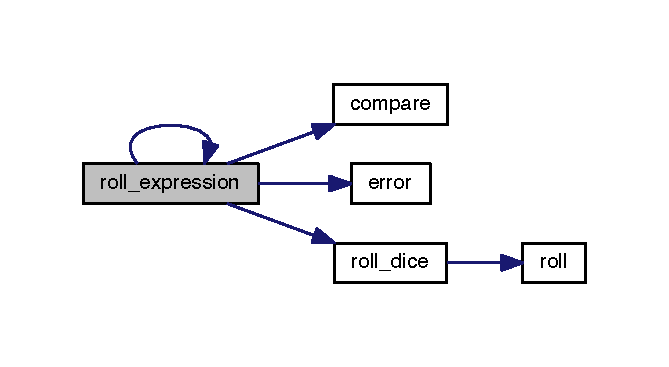
\includegraphics[width=321pt]{roll_8c_ad4c76f688ad79c99d3c39f54358964c8_cgraph}
\end{center}
\end{figure}




\subsection{Variable Documentation}
\hypertarget{roll_8c_ab1b14e1b3006d5f4665e1f5a74e25f93}{}\index{roll.\+c@{roll.\+c}!positive\+\_\+flag@{positive\+\_\+flag}}
\index{positive\+\_\+flag@{positive\+\_\+flag}!roll.\+c@{roll.\+c}}
\subsubsection[{positive\+\_\+flag}]{\setlength{\rightskip}{0pt plus 5cm}int positive\+\_\+flag}\label{roll_8c_ab1b14e1b3006d5f4665e1f5a74e25f93}
command line argument\+: allow only positive results 

Referenced by main().

\hypertarget{roll_8c_abec29e6443957b8a01502b04f2e9ba39}{}\index{roll.\+c@{roll.\+c}!sum\+\_\+flag@{sum\+\_\+flag}}
\index{sum\+\_\+flag@{sum\+\_\+flag}!roll.\+c@{roll.\+c}}
\subsubsection[{sum\+\_\+flag}]{\setlength{\rightskip}{0pt plus 5cm}int sum\+\_\+flag = {\bf F\+A\+L\+S\+E}}\label{roll_8c_abec29e6443957b8a01502b04f2e9ba39}
command line argument\+: sum series 

Definition at line 16 of file roll.\+c.



Referenced by main().

\hypertarget{roll_8c_a4c7699f4d1b8ee152b8d35bbc579430b}{}\index{roll.\+c@{roll.\+c}!verbose\+\_\+flag@{verbose\+\_\+flag}}
\index{verbose\+\_\+flag@{verbose\+\_\+flag}!roll.\+c@{roll.\+c}}
\subsubsection[{verbose\+\_\+flag}]{\setlength{\rightskip}{0pt plus 5cm}int verbose\+\_\+flag = {\bf F\+A\+L\+S\+E}\hspace{0.3cm}{\ttfamily [static]}}\label{roll_8c_a4c7699f4d1b8ee152b8d35bbc579430b}
command line argument\+: verbose output 

Definition at line 17 of file roll.\+c.



Referenced by main(), and roll\+\_\+dice().

\hypertarget{roll_8c_a541cb25faf92a00e9ecaa761baed4c2f}{}\index{roll.\+c@{roll.\+c}!version\+\_\+flag@{version\+\_\+flag}}
\index{version\+\_\+flag@{version\+\_\+flag}!roll.\+c@{roll.\+c}}
\subsubsection[{version\+\_\+flag}]{\setlength{\rightskip}{0pt plus 5cm}int version\+\_\+flag = {\bf F\+A\+L\+S\+E}\hspace{0.3cm}{\ttfamily [static]}}\label{roll_8c_a541cb25faf92a00e9ecaa761baed4c2f}
command line argument\+: version 

Definition at line 18 of file roll.\+c.



Referenced by main().


\hypertarget{roll_8h}{}\section{roll.\+h File Reference}
\label{roll_8h}\index{roll.\+h@{roll.\+h}}


The main include file.  


{\ttfamily \#include $<$stdio.\+h$>$}\\*
{\ttfamily \#include $<$stdlib.\+h$>$}\\*
{\ttfamily \#include $<$strings.\+h$>$}\\*
{\ttfamily \#include $<$string.\+h$>$}\\*
{\ttfamily \#include $<$getopt.\+h$>$}\\*
{\ttfamily \#include $<$errno.\+h$>$}\\*
{\ttfamily \#include $<$time.\+h$>$}\\*
{\ttfamily \#include $<$math.\+h$>$}\\*
{\ttfamily \#include $<$limits.\+h$>$}\\*
{\ttfamily \#include \char`\"{}config.\+h\char`\"{}}\\*
Include dependency graph for roll.\+h\+:
\nopagebreak
\begin{figure}[H]
\begin{center}
\leavevmode
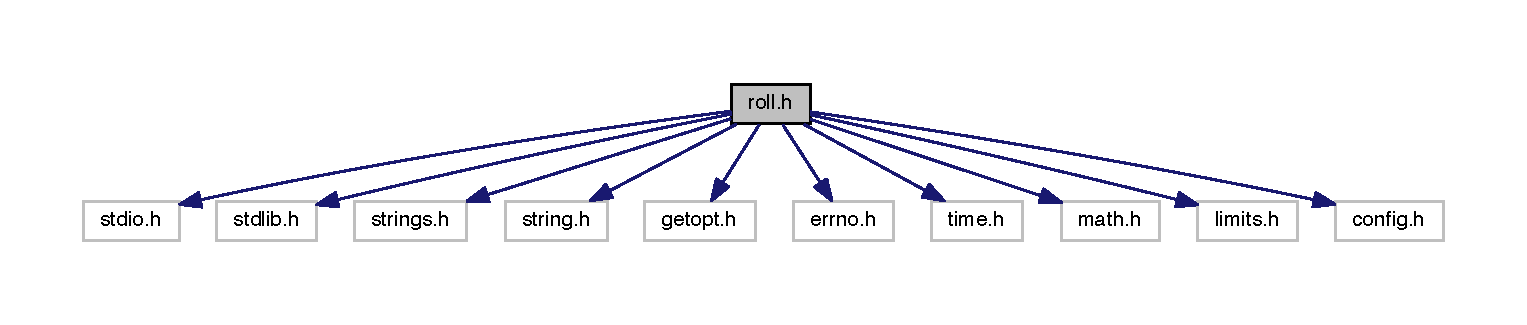
\includegraphics[width=350pt]{roll_8h__incl}
\end{center}
\end{figure}
This graph shows which files directly or indirectly include this file\+:
\nopagebreak
\begin{figure}[H]
\begin{center}
\leavevmode
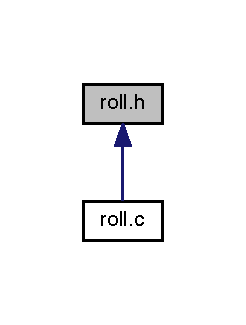
\includegraphics[width=118pt]{roll_8h__dep__incl}
\end{center}
\end{figure}
\subsection*{Data Structures}
\begin{DoxyCompactItemize}
\item 
struct \hyperlink{structir__node}{ir\+\_\+node}
\begin{DoxyCompactList}\small\item\em node of the intermediate representation parse tree \end{DoxyCompactList}\end{DoxyCompactItemize}
\subsection*{Macros}
\begin{DoxyCompactItemize}
\item 
\#define \hyperlink{roll_8h_ae05abae0cdd75043c8e635c5c90f9272}{E\+X\+P\+R\+E\+S\+S\+I\+O\+N\+\_\+\+S\+I\+Z\+E}~1024
\item 
\#define \hyperlink{roll_8h_aa93f0eb578d23995850d61f7d61c55c1}{F\+A\+L\+S\+E}~0
\item 
\#define \hyperlink{roll_8h_a625dac461fbab83b1c1d04f3aceeb8f3}{H\+U\+N\+D\+R\+E\+D}~-\/1
\item 
\#define \hyperlink{roll_8h_ac22133e25cbb119a03e18be7e2b029f4}{O\+P\+\_\+\+D\+I\+C\+E}~4
\item 
\#define \hyperlink{roll_8h_addec4be73478fb9243f0ea0087366641}{O\+P\+\_\+\+D\+I\+V}~3
\item 
\#define \hyperlink{roll_8h_a81d577022941aa88aac9f64eef8d7faf}{O\+P\+\_\+\+G\+E}~10
\item 
\#define \hyperlink{roll_8h_a0fa482032824fe178a5c8510a6b268e8}{O\+P\+\_\+\+G\+T}~9
\item 
\#define \hyperlink{roll_8h_ab9cc57ec763eabfbcdc422bcd574d50b}{O\+P\+\_\+\+H\+I\+G\+H}~7
\item 
\#define \hyperlink{roll_8h_ae26997ae51e5ac9ad3717d9010ef9c92}{O\+P\+\_\+\+L\+E}~12
\item 
\#define \hyperlink{roll_8h_a8db1c769c2173f00e38f457c2d6450c0}{O\+P\+\_\+\+L\+O\+W}~8
\item 
\#define \hyperlink{roll_8h_a09b4bd252d4ef2d01ba2394ce89096eb}{O\+P\+\_\+\+L\+T}~11
\item 
\#define \hyperlink{roll_8h_ab62390fc8d7f39a0edfd26f5c30df780}{O\+P\+\_\+\+M\+I\+N\+U\+S}~6
\item 
\#define \hyperlink{roll_8h_ad00f801ce58135d1943ecd405054941d}{O\+P\+\_\+\+N\+E}~13
\item 
\#define \hyperlink{roll_8h_aee5d81dd03df6e8030c9f559ec346f95}{O\+P\+\_\+\+N\+U\+M\+B\+E\+R}~1
\item 
\#define \hyperlink{roll_8h_a75a9903938da31e530a136d37a839848}{O\+P\+\_\+\+P\+L\+U\+S}~5
\item 
\#define \hyperlink{roll_8h_abb555c8b38c708a0dd1c0a51849ce240}{O\+P\+\_\+\+R\+E\+P}~14
\item 
\#define \hyperlink{roll_8h_ac574cdf3dd634e54040f68400ec26e48}{O\+P\+\_\+\+T\+I\+M\+E\+S}~2
\item 
\#define \hyperlink{roll_8h_af3bc8a5595302da2f2984141e633266f}{srandomdev}()~srand((unsigned) time(N\+U\+L\+L))
\item 
\#define \hyperlink{roll_8h_aa8cecfc5c5c054d2875c03e77b7be15d}{T\+R\+U\+E}~1
\end{DoxyCompactItemize}
\subsection*{Functions}
\begin{DoxyCompactItemize}
\item 
struct \hyperlink{structir__node}{ir\+\_\+node} $\ast$ \hyperlink{roll_8h_ab19c6534375437b3fa360f51198028f5}{allocate\+\_\+node} (void)
\begin{DoxyCompactList}\small\item\em Allocates a new I\+R node. \end{DoxyCompactList}\item 
void \hyperlink{roll_8h_a8e1bf3d5ea0a885f81e71d2023a55777}{error} (char $\ast$message)
\begin{DoxyCompactList}\small\item\em Prints the specified error message and exits with a failure status. \end{DoxyCompactList}\item 
struct \hyperlink{structir__node}{ir\+\_\+node} $\ast$ \hyperlink{roll_8h_aa255c368423347571a5a7ec8a01840cd}{new\+\_\+dice} (struct \hyperlink{structir__node}{ir\+\_\+node} $\ast$sides)
\begin{DoxyCompactList}\small\item\em Allocates a new D\+I\+C\+E node. \end{DoxyCompactList}\item 
struct \hyperlink{structir__node}{ir\+\_\+node} $\ast$ \hyperlink{roll_8h_a9708fd7a304b37bac39a25b0a8fe889e}{new\+\_\+number} (int number)
\begin{DoxyCompactList}\small\item\em Allocates a new N\+U\+M\+B\+E\+R node. \end{DoxyCompactList}\item 
struct \hyperlink{structir__node}{ir\+\_\+node} $\ast$ \hyperlink{roll_8h_ad29ccfc41dabb89e317de25329c3d279}{new\+\_\+op} (unsigned short int op, struct \hyperlink{structir__node}{ir\+\_\+node} $\ast$left, struct \hyperlink{structir__node}{ir\+\_\+node} $\ast$right)
\begin{DoxyCompactList}\small\item\em Allocates a new O\+P node. \end{DoxyCompactList}\item 
int \hyperlink{roll_8h_a25887d1873a9df6c717c4daae7d4efc2}{roll} (int dice)
\begin{DoxyCompactList}\small\item\em Rolls an n-\/sided dice. \end{DoxyCompactList}\item 
int \hyperlink{roll_8h_ad4c76f688ad79c99d3c39f54358964c8}{roll\+\_\+expression} (struct \hyperlink{structir__node}{ir\+\_\+node} $\ast$node, int print)
\begin{DoxyCompactList}\small\item\em Roll dices and compute expressions. \end{DoxyCompactList}\item 
\hypertarget{roll_8h_a2ef30c42cbc289d899a8be5d2d8f77d0}{}void \hyperlink{roll_8h_a2ef30c42cbc289d899a8be5d2d8f77d0}{usage} ()\label{roll_8h_a2ef30c42cbc289d899a8be5d2d8f77d0}

\begin{DoxyCompactList}\small\item\em Prints the program\textquotesingle{}s usage. \end{DoxyCompactList}\end{DoxyCompactItemize}


\subsection{Detailed Description}
The main include file. 

\begin{DoxyAuthor}{Author}
Matteo Corti 
\end{DoxyAuthor}


\subsection{Macro Definition Documentation}
\hypertarget{roll_8h_ae05abae0cdd75043c8e635c5c90f9272}{}\index{roll.\+h@{roll.\+h}!E\+X\+P\+R\+E\+S\+S\+I\+O\+N\+\_\+\+S\+I\+Z\+E@{E\+X\+P\+R\+E\+S\+S\+I\+O\+N\+\_\+\+S\+I\+Z\+E}}
\index{E\+X\+P\+R\+E\+S\+S\+I\+O\+N\+\_\+\+S\+I\+Z\+E@{E\+X\+P\+R\+E\+S\+S\+I\+O\+N\+\_\+\+S\+I\+Z\+E}!roll.\+h@{roll.\+h}}
\subsubsection[{E\+X\+P\+R\+E\+S\+S\+I\+O\+N\+\_\+\+S\+I\+Z\+E}]{\setlength{\rightskip}{0pt plus 5cm}\#define E\+X\+P\+R\+E\+S\+S\+I\+O\+N\+\_\+\+S\+I\+Z\+E~1024}\label{roll_8h_ae05abae0cdd75043c8e635c5c90f9272}
\begin{DoxyRefDesc}{Todo}
\item[\hyperlink{todo__todo000001}{Todo}]The maximum expression length should be dynamic \end{DoxyRefDesc}
Maximum expression length 

Definition at line 40 of file roll.\+h.



Referenced by main().

\hypertarget{roll_8h_aa93f0eb578d23995850d61f7d61c55c1}{}\index{roll.\+h@{roll.\+h}!F\+A\+L\+S\+E@{F\+A\+L\+S\+E}}
\index{F\+A\+L\+S\+E@{F\+A\+L\+S\+E}!roll.\+h@{roll.\+h}}
\subsubsection[{F\+A\+L\+S\+E}]{\setlength{\rightskip}{0pt plus 5cm}\#define F\+A\+L\+S\+E~0}\label{roll_8h_aa93f0eb578d23995850d61f7d61c55c1}
Boolean false 

Definition at line 33 of file roll.\+h.



Referenced by roll\+\_\+expression().

\hypertarget{roll_8h_a625dac461fbab83b1c1d04f3aceeb8f3}{}\index{roll.\+h@{roll.\+h}!H\+U\+N\+D\+R\+E\+D@{H\+U\+N\+D\+R\+E\+D}}
\index{H\+U\+N\+D\+R\+E\+D@{H\+U\+N\+D\+R\+E\+D}!roll.\+h@{roll.\+h}}
\subsubsection[{H\+U\+N\+D\+R\+E\+D}]{\setlength{\rightskip}{0pt plus 5cm}\#define H\+U\+N\+D\+R\+E\+D~-\/1}\label{roll_8h_a625dac461fbab83b1c1d04f3aceeb8f3}
Constant representing a 1d100 rolled with 1d10 for the units and 1d10 for the tens 

Definition at line 45 of file roll.\+h.



Referenced by roll\+\_\+dice().

\hypertarget{roll_8h_ac22133e25cbb119a03e18be7e2b029f4}{}\index{roll.\+h@{roll.\+h}!O\+P\+\_\+\+D\+I\+C\+E@{O\+P\+\_\+\+D\+I\+C\+E}}
\index{O\+P\+\_\+\+D\+I\+C\+E@{O\+P\+\_\+\+D\+I\+C\+E}!roll.\+h@{roll.\+h}}
\subsubsection[{O\+P\+\_\+\+D\+I\+C\+E}]{\setlength{\rightskip}{0pt plus 5cm}\#define O\+P\+\_\+\+D\+I\+C\+E~4}\label{roll_8h_ac22133e25cbb119a03e18be7e2b029f4}
N-\/sided dice node 

Definition at line 83 of file roll.\+h.



Referenced by new\+\_\+dice(), and roll\+\_\+expression().

\hypertarget{roll_8h_addec4be73478fb9243f0ea0087366641}{}\index{roll.\+h@{roll.\+h}!O\+P\+\_\+\+D\+I\+V@{O\+P\+\_\+\+D\+I\+V}}
\index{O\+P\+\_\+\+D\+I\+V@{O\+P\+\_\+\+D\+I\+V}!roll.\+h@{roll.\+h}}
\subsubsection[{O\+P\+\_\+\+D\+I\+V}]{\setlength{\rightskip}{0pt plus 5cm}\#define O\+P\+\_\+\+D\+I\+V~3}\label{roll_8h_addec4be73478fb9243f0ea0087366641}
Integer division node 

Definition at line 82 of file roll.\+h.



Referenced by roll\+\_\+expression().

\hypertarget{roll_8h_a81d577022941aa88aac9f64eef8d7faf}{}\index{roll.\+h@{roll.\+h}!O\+P\+\_\+\+G\+E@{O\+P\+\_\+\+G\+E}}
\index{O\+P\+\_\+\+G\+E@{O\+P\+\_\+\+G\+E}!roll.\+h@{roll.\+h}}
\subsubsection[{O\+P\+\_\+\+G\+E}]{\setlength{\rightskip}{0pt plus 5cm}\#define O\+P\+\_\+\+G\+E~10}\label{roll_8h_a81d577022941aa88aac9f64eef8d7faf}
Keep results greater or equal than 

Definition at line 89 of file roll.\+h.



Referenced by roll\+\_\+expression().

\hypertarget{roll_8h_a0fa482032824fe178a5c8510a6b268e8}{}\index{roll.\+h@{roll.\+h}!O\+P\+\_\+\+G\+T@{O\+P\+\_\+\+G\+T}}
\index{O\+P\+\_\+\+G\+T@{O\+P\+\_\+\+G\+T}!roll.\+h@{roll.\+h}}
\subsubsection[{O\+P\+\_\+\+G\+T}]{\setlength{\rightskip}{0pt plus 5cm}\#define O\+P\+\_\+\+G\+T~9}\label{roll_8h_a0fa482032824fe178a5c8510a6b268e8}
Keep results greater than 

Definition at line 88 of file roll.\+h.



Referenced by roll\+\_\+expression().

\hypertarget{roll_8h_ab9cc57ec763eabfbcdc422bcd574d50b}{}\index{roll.\+h@{roll.\+h}!O\+P\+\_\+\+H\+I\+G\+H@{O\+P\+\_\+\+H\+I\+G\+H}}
\index{O\+P\+\_\+\+H\+I\+G\+H@{O\+P\+\_\+\+H\+I\+G\+H}!roll.\+h@{roll.\+h}}
\subsubsection[{O\+P\+\_\+\+H\+I\+G\+H}]{\setlength{\rightskip}{0pt plus 5cm}\#define O\+P\+\_\+\+H\+I\+G\+H~7}\label{roll_8h_ab9cc57ec763eabfbcdc422bcd574d50b}
Keep highest results node 

Definition at line 86 of file roll.\+h.



Referenced by roll\+\_\+expression().

\hypertarget{roll_8h_ae26997ae51e5ac9ad3717d9010ef9c92}{}\index{roll.\+h@{roll.\+h}!O\+P\+\_\+\+L\+E@{O\+P\+\_\+\+L\+E}}
\index{O\+P\+\_\+\+L\+E@{O\+P\+\_\+\+L\+E}!roll.\+h@{roll.\+h}}
\subsubsection[{O\+P\+\_\+\+L\+E}]{\setlength{\rightskip}{0pt plus 5cm}\#define O\+P\+\_\+\+L\+E~12}\label{roll_8h_ae26997ae51e5ac9ad3717d9010ef9c92}
Keep results less or equal than 

Definition at line 91 of file roll.\+h.



Referenced by roll\+\_\+expression().

\hypertarget{roll_8h_a8db1c769c2173f00e38f457c2d6450c0}{}\index{roll.\+h@{roll.\+h}!O\+P\+\_\+\+L\+O\+W@{O\+P\+\_\+\+L\+O\+W}}
\index{O\+P\+\_\+\+L\+O\+W@{O\+P\+\_\+\+L\+O\+W}!roll.\+h@{roll.\+h}}
\subsubsection[{O\+P\+\_\+\+L\+O\+W}]{\setlength{\rightskip}{0pt plus 5cm}\#define O\+P\+\_\+\+L\+O\+W~8}\label{roll_8h_a8db1c769c2173f00e38f457c2d6450c0}
Keep lowest resutls node 

Definition at line 87 of file roll.\+h.



Referenced by roll\+\_\+expression().

\hypertarget{roll_8h_a09b4bd252d4ef2d01ba2394ce89096eb}{}\index{roll.\+h@{roll.\+h}!O\+P\+\_\+\+L\+T@{O\+P\+\_\+\+L\+T}}
\index{O\+P\+\_\+\+L\+T@{O\+P\+\_\+\+L\+T}!roll.\+h@{roll.\+h}}
\subsubsection[{O\+P\+\_\+\+L\+T}]{\setlength{\rightskip}{0pt plus 5cm}\#define O\+P\+\_\+\+L\+T~11}\label{roll_8h_a09b4bd252d4ef2d01ba2394ce89096eb}
Keep results less than 

Definition at line 90 of file roll.\+h.



Referenced by roll\+\_\+expression().

\hypertarget{roll_8h_ab62390fc8d7f39a0edfd26f5c30df780}{}\index{roll.\+h@{roll.\+h}!O\+P\+\_\+\+M\+I\+N\+U\+S@{O\+P\+\_\+\+M\+I\+N\+U\+S}}
\index{O\+P\+\_\+\+M\+I\+N\+U\+S@{O\+P\+\_\+\+M\+I\+N\+U\+S}!roll.\+h@{roll.\+h}}
\subsubsection[{O\+P\+\_\+\+M\+I\+N\+U\+S}]{\setlength{\rightskip}{0pt plus 5cm}\#define O\+P\+\_\+\+M\+I\+N\+U\+S~6}\label{roll_8h_ab62390fc8d7f39a0edfd26f5c30df780}
Subtraction node 

Definition at line 85 of file roll.\+h.



Referenced by roll\+\_\+expression().

\hypertarget{roll_8h_ad00f801ce58135d1943ecd405054941d}{}\index{roll.\+h@{roll.\+h}!O\+P\+\_\+\+N\+E@{O\+P\+\_\+\+N\+E}}
\index{O\+P\+\_\+\+N\+E@{O\+P\+\_\+\+N\+E}!roll.\+h@{roll.\+h}}
\subsubsection[{O\+P\+\_\+\+N\+E}]{\setlength{\rightskip}{0pt plus 5cm}\#define O\+P\+\_\+\+N\+E~13}\label{roll_8h_ad00f801ce58135d1943ecd405054941d}
Keep results different from 

Definition at line 92 of file roll.\+h.



Referenced by roll\+\_\+expression().

\hypertarget{roll_8h_aee5d81dd03df6e8030c9f559ec346f95}{}\index{roll.\+h@{roll.\+h}!O\+P\+\_\+\+N\+U\+M\+B\+E\+R@{O\+P\+\_\+\+N\+U\+M\+B\+E\+R}}
\index{O\+P\+\_\+\+N\+U\+M\+B\+E\+R@{O\+P\+\_\+\+N\+U\+M\+B\+E\+R}!roll.\+h@{roll.\+h}}
\subsubsection[{O\+P\+\_\+\+N\+U\+M\+B\+E\+R}]{\setlength{\rightskip}{0pt plus 5cm}\#define O\+P\+\_\+\+N\+U\+M\+B\+E\+R~1}\label{roll_8h_aee5d81dd03df6e8030c9f559ec346f95}
Number node 

Definition at line 80 of file roll.\+h.



Referenced by new\+\_\+number(), and roll\+\_\+expression().

\hypertarget{roll_8h_a75a9903938da31e530a136d37a839848}{}\index{roll.\+h@{roll.\+h}!O\+P\+\_\+\+P\+L\+U\+S@{O\+P\+\_\+\+P\+L\+U\+S}}
\index{O\+P\+\_\+\+P\+L\+U\+S@{O\+P\+\_\+\+P\+L\+U\+S}!roll.\+h@{roll.\+h}}
\subsubsection[{O\+P\+\_\+\+P\+L\+U\+S}]{\setlength{\rightskip}{0pt plus 5cm}\#define O\+P\+\_\+\+P\+L\+U\+S~5}\label{roll_8h_a75a9903938da31e530a136d37a839848}
Addition node 

Definition at line 84 of file roll.\+h.



Referenced by roll\+\_\+expression().

\hypertarget{roll_8h_abb555c8b38c708a0dd1c0a51849ce240}{}\index{roll.\+h@{roll.\+h}!O\+P\+\_\+\+R\+E\+P@{O\+P\+\_\+\+R\+E\+P}}
\index{O\+P\+\_\+\+R\+E\+P@{O\+P\+\_\+\+R\+E\+P}!roll.\+h@{roll.\+h}}
\subsubsection[{O\+P\+\_\+\+R\+E\+P}]{\setlength{\rightskip}{0pt plus 5cm}\#define O\+P\+\_\+\+R\+E\+P~14}\label{roll_8h_abb555c8b38c708a0dd1c0a51849ce240}
Number of rolls (repetitions) 

Definition at line 93 of file roll.\+h.



Referenced by roll\+\_\+expression().

\hypertarget{roll_8h_ac574cdf3dd634e54040f68400ec26e48}{}\index{roll.\+h@{roll.\+h}!O\+P\+\_\+\+T\+I\+M\+E\+S@{O\+P\+\_\+\+T\+I\+M\+E\+S}}
\index{O\+P\+\_\+\+T\+I\+M\+E\+S@{O\+P\+\_\+\+T\+I\+M\+E\+S}!roll.\+h@{roll.\+h}}
\subsubsection[{O\+P\+\_\+\+T\+I\+M\+E\+S}]{\setlength{\rightskip}{0pt plus 5cm}\#define O\+P\+\_\+\+T\+I\+M\+E\+S~2}\label{roll_8h_ac574cdf3dd634e54040f68400ec26e48}
Multiplication node 

Definition at line 81 of file roll.\+h.



Referenced by roll\+\_\+expression().

\hypertarget{roll_8h_af3bc8a5595302da2f2984141e633266f}{}\index{roll.\+h@{roll.\+h}!srandomdev@{srandomdev}}
\index{srandomdev@{srandomdev}!roll.\+h@{roll.\+h}}
\subsubsection[{srandomdev}]{\setlength{\rightskip}{0pt plus 5cm}\#define srandomdev(
\begin{DoxyParamCaption}
{}
\end{DoxyParamCaption}
)~srand((unsigned) time(N\+U\+L\+L))}\label{roll_8h_af3bc8a5595302da2f2984141e633266f}
defines srandomdev usig srand of the current time if srandomdev and getpid are missing 

Definition at line 72 of file roll.\+h.



Referenced by main().

\hypertarget{roll_8h_aa8cecfc5c5c054d2875c03e77b7be15d}{}\index{roll.\+h@{roll.\+h}!T\+R\+U\+E@{T\+R\+U\+E}}
\index{T\+R\+U\+E@{T\+R\+U\+E}!roll.\+h@{roll.\+h}}
\subsubsection[{T\+R\+U\+E}]{\setlength{\rightskip}{0pt plus 5cm}\#define T\+R\+U\+E~1}\label{roll_8h_aa8cecfc5c5c054d2875c03e77b7be15d}
Boolean true 

Definition at line 28 of file roll.\+h.



Referenced by main(), and roll\+\_\+expression().



\subsection{Function Documentation}
\hypertarget{roll_8h_ab19c6534375437b3fa360f51198028f5}{}\index{roll.\+h@{roll.\+h}!allocate\+\_\+node@{allocate\+\_\+node}}
\index{allocate\+\_\+node@{allocate\+\_\+node}!roll.\+h@{roll.\+h}}
\subsubsection[{allocate\+\_\+node(void)}]{\setlength{\rightskip}{0pt plus 5cm}struct {\bf ir\+\_\+node}$\ast$ allocate\+\_\+node (
\begin{DoxyParamCaption}
\item[{void}]{}
\end{DoxyParamCaption}
)}\label{roll_8h_ab19c6534375437b3fa360f51198028f5}


Allocates a new I\+R node. 

\begin{DoxyReturn}{Returns}
Newly allocated node 
\end{DoxyReturn}


Definition at line 266 of file roll.\+c.



References error(), ir\+\_\+node\+::left, ir\+\_\+node\+::next, ir\+\_\+node\+::op, ir\+\_\+node\+::right, and ir\+\_\+node\+::value.



Referenced by new\+\_\+dice(), new\+\_\+number(), and new\+\_\+op().


\begin{DoxyCode}
266                                          \{
267 
268   \textcolor{keyword}{struct }\hyperlink{structir__node}{ir\_node} * node = malloc(\textcolor{keyword}{sizeof}(\textcolor{keyword}{struct} \hyperlink{structir__node}{ir\_node}));
269   \textcolor{keywordflow}{if} (node == NULL) \{
270     \hyperlink{roll_8c_a8e1bf3d5ea0a885f81e71d2023a55777}{error}(\textcolor{stringliteral}{"Out of memory\(\backslash\)n"});
271     exit(EXIT\_FAILURE);
272   \}
273 
274   \textcolor{comment}{/* initialize default values */}
275   node->\hyperlink{structir__node_ab6ecf53bf92c825b620435fc93a6b6ee}{left}  = NULL;
276   node->\hyperlink{structir__node_ab72283b06a90004232c315bc52b0e9b5}{right} = NULL;
277   node->\hyperlink{structir__node_ab1d37e8ddfafb50b2633b66af37fb064}{next}  = NULL;
278   node->\hyperlink{structir__node_a4d977601c157f732bd7655d7a47e8545}{op}    = 0;
279   node->\hyperlink{structir__node_a4cd43e9ea9717dc8bda34aa8ca5f8d35}{value} = 0;
280   
281   \textcolor{keywordflow}{return} node;
282   
283 \}
\end{DoxyCode}


Here is the call graph for this function\+:
\nopagebreak
\begin{figure}[H]
\begin{center}
\leavevmode
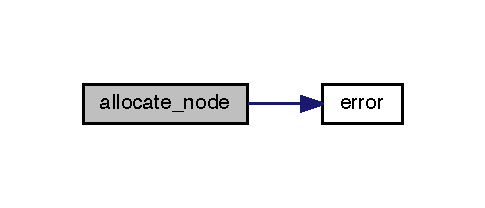
\includegraphics[width=233pt]{roll_8h_ab19c6534375437b3fa360f51198028f5_cgraph}
\end{center}
\end{figure}


\hypertarget{roll_8h_a8e1bf3d5ea0a885f81e71d2023a55777}{}\index{roll.\+h@{roll.\+h}!error@{error}}
\index{error@{error}!roll.\+h@{roll.\+h}}
\subsubsection[{error(char $\ast$message)}]{\setlength{\rightskip}{0pt plus 5cm}void error (
\begin{DoxyParamCaption}
\item[{char $\ast$}]{message}
\end{DoxyParamCaption}
)}\label{roll_8h_a8e1bf3d5ea0a885f81e71d2023a55777}


Prints the specified error message and exits with a failure status. 


\begin{DoxyParams}{Parameters}
{\em } & \\
\hline
\end{DoxyParams}


Definition at line 50 of file roll.\+c.



Referenced by allocate\+\_\+node(), main(), and roll\+\_\+expression().


\begin{DoxyCode}
50                            \{
51   fprintf(stderr, \textcolor{stringliteral}{"\(\backslash\)nError: %s\(\backslash\)n"}, message);
52   exit(EXIT\_FAILURE);
53 \}
\end{DoxyCode}
\hypertarget{roll_8h_aa255c368423347571a5a7ec8a01840cd}{}\index{roll.\+h@{roll.\+h}!new\+\_\+dice@{new\+\_\+dice}}
\index{new\+\_\+dice@{new\+\_\+dice}!roll.\+h@{roll.\+h}}
\subsubsection[{new\+\_\+dice(struct ir\+\_\+node $\ast$sides)}]{\setlength{\rightskip}{0pt plus 5cm}struct {\bf ir\+\_\+node}$\ast$ new\+\_\+dice (
\begin{DoxyParamCaption}
\item[{struct {\bf ir\+\_\+node} $\ast$}]{sides}
\end{DoxyParamCaption}
)}\label{roll_8h_aa255c368423347571a5a7ec8a01840cd}


Allocates a new D\+I\+C\+E node. 


\begin{DoxyParams}{Parameters}
{\em } & \\
\hline
\end{DoxyParams}


Definition at line 344 of file roll.\+c.



References allocate\+\_\+node(), ir\+\_\+node\+::op, O\+P\+\_\+\+D\+I\+C\+E, ir\+\_\+node\+::right, and ir\+\_\+node\+::value.


\begin{DoxyCode}
344                                                     \{
345   
346   \textcolor{keyword}{struct }\hyperlink{structir__node}{ir\_node} * node = \hyperlink{roll_8c_ab19c6534375437b3fa360f51198028f5}{allocate\_node}();
347   node->\hyperlink{structir__node_a4d977601c157f732bd7655d7a47e8545}{op}    = \hyperlink{roll_8h_ac22133e25cbb119a03e18be7e2b029f4}{OP\_DICE};
348   node->\hyperlink{structir__node_a4cd43e9ea9717dc8bda34aa8ca5f8d35}{value} = 0;
349   node->\hyperlink{structir__node_ab72283b06a90004232c315bc52b0e9b5}{right} = sides;
350   \textcolor{keywordflow}{return} node;
351   
352 \}
\end{DoxyCode}


Here is the call graph for this function\+:
\nopagebreak
\begin{figure}[H]
\begin{center}
\leavevmode
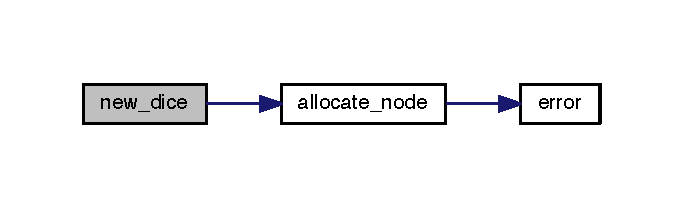
\includegraphics[width=328pt]{roll_8h_aa255c368423347571a5a7ec8a01840cd_cgraph}
\end{center}
\end{figure}


\hypertarget{roll_8h_a9708fd7a304b37bac39a25b0a8fe889e}{}\index{roll.\+h@{roll.\+h}!new\+\_\+number@{new\+\_\+number}}
\index{new\+\_\+number@{new\+\_\+number}!roll.\+h@{roll.\+h}}
\subsubsection[{new\+\_\+number(int number)}]{\setlength{\rightskip}{0pt plus 5cm}struct {\bf ir\+\_\+node}$\ast$ new\+\_\+number (
\begin{DoxyParamCaption}
\item[{int}]{number}
\end{DoxyParamCaption}
)}\label{roll_8h_a9708fd7a304b37bac39a25b0a8fe889e}


Allocates a new N\+U\+M\+B\+E\+R node. 


\begin{DoxyParams}{Parameters}
{\em } & \\
\hline
\end{DoxyParams}


Definition at line 290 of file roll.\+c.



References allocate\+\_\+node(), ir\+\_\+node\+::op, O\+P\+\_\+\+N\+U\+M\+B\+E\+R, and ir\+\_\+node\+::value.


\begin{DoxyCode}
290                                            \{
291 
292   \textcolor{keyword}{struct }\hyperlink{structir__node}{ir\_node} * node = \hyperlink{roll_8c_ab19c6534375437b3fa360f51198028f5}{allocate\_node}();
293   node->\hyperlink{structir__node_a4d977601c157f732bd7655d7a47e8545}{op}    = \hyperlink{roll_8h_aee5d81dd03df6e8030c9f559ec346f95}{OP\_NUMBER};
294   node->\hyperlink{structir__node_a4cd43e9ea9717dc8bda34aa8ca5f8d35}{value} = number;
295 
296   \textcolor{keywordflow}{return} node;
297 
298 \}
\end{DoxyCode}


Here is the call graph for this function\+:
\nopagebreak
\begin{figure}[H]
\begin{center}
\leavevmode
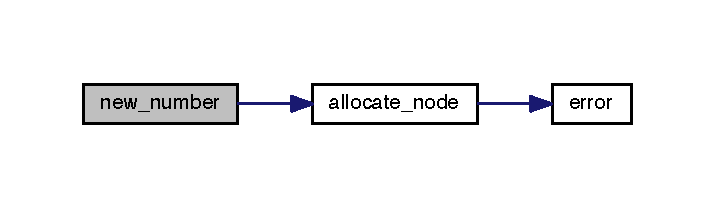
\includegraphics[width=343pt]{roll_8h_a9708fd7a304b37bac39a25b0a8fe889e_cgraph}
\end{center}
\end{figure}


\hypertarget{roll_8h_ad29ccfc41dabb89e317de25329c3d279}{}\index{roll.\+h@{roll.\+h}!new\+\_\+op@{new\+\_\+op}}
\index{new\+\_\+op@{new\+\_\+op}!roll.\+h@{roll.\+h}}
\subsubsection[{new\+\_\+op(unsigned short int op, struct ir\+\_\+node $\ast$left, struct ir\+\_\+node $\ast$right)}]{\setlength{\rightskip}{0pt plus 5cm}struct {\bf ir\+\_\+node}$\ast$ new\+\_\+op (
\begin{DoxyParamCaption}
\item[{unsigned short int}]{op, }
\item[{struct {\bf ir\+\_\+node} $\ast$}]{left, }
\item[{struct {\bf ir\+\_\+node} $\ast$}]{right}
\end{DoxyParamCaption}
)}\label{roll_8h_ad29ccfc41dabb89e317de25329c3d279}


Allocates a new O\+P node. 


\begin{DoxyParams}{Parameters}
{\em } & \\
\hline
\end{DoxyParams}


Definition at line 328 of file roll.\+c.



References allocate\+\_\+node(), ir\+\_\+node\+::left, ir\+\_\+node\+::op, ir\+\_\+node\+::right, and ir\+\_\+node\+::value.


\begin{DoxyCode}
328                                                                                                 \{
329 
330   \textcolor{keyword}{struct }\hyperlink{structir__node}{ir\_node} * node = \hyperlink{roll_8c_ab19c6534375437b3fa360f51198028f5}{allocate\_node}();
331   node->\hyperlink{structir__node_a4d977601c157f732bd7655d7a47e8545}{op}    = \hyperlink{structir__node_a4d977601c157f732bd7655d7a47e8545}{op};
332   node->\hyperlink{structir__node_a4cd43e9ea9717dc8bda34aa8ca5f8d35}{value} = 0;
333   node->\hyperlink{structir__node_ab6ecf53bf92c825b620435fc93a6b6ee}{left}  = \hyperlink{structir__node_ab6ecf53bf92c825b620435fc93a6b6ee}{left};
334   node->\hyperlink{structir__node_ab72283b06a90004232c315bc52b0e9b5}{right} = \hyperlink{structir__node_ab72283b06a90004232c315bc52b0e9b5}{right};
335   \textcolor{keywordflow}{return} node;
336   
337 \}
\end{DoxyCode}


Here is the call graph for this function\+:
\nopagebreak
\begin{figure}[H]
\begin{center}
\leavevmode
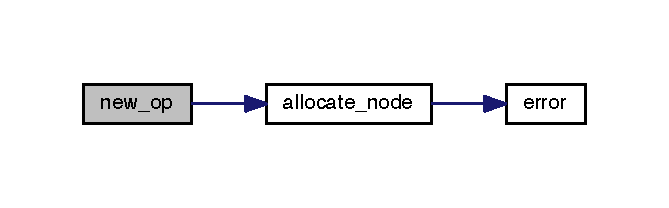
\includegraphics[width=321pt]{roll_8h_ad29ccfc41dabb89e317de25329c3d279_cgraph}
\end{center}
\end{figure}


\hypertarget{roll_8h_a25887d1873a9df6c717c4daae7d4efc2}{}\index{roll.\+h@{roll.\+h}!roll@{roll}}
\index{roll@{roll}!roll.\+h@{roll.\+h}}
\subsubsection[{roll(int dice)}]{\setlength{\rightskip}{0pt plus 5cm}int roll (
\begin{DoxyParamCaption}
\item[{int}]{dice}
\end{DoxyParamCaption}
)}\label{roll_8h_a25887d1873a9df6c717c4daae7d4efc2}


Rolls an n-\/sided dice. 


\begin{DoxyParams}{Parameters}
{\em } & \\
\hline
\end{DoxyParams}


Definition at line 124 of file roll.\+c.



Referenced by roll\+\_\+dice().


\begin{DoxyCode}
124                    \{
125 
126   \textcolor{comment}{/* }
127 \textcolor{comment}{   * In: W. H. Press et al,Numerical Recipes in C: The Art of}
128 \textcolor{comment}{   * Scientific Computing.  New York, Cambridge University Press,}
129 \textcolor{comment}{   * 1992, 2nd ed., p. 277}
130 \textcolor{comment}{   *}
131 \textcolor{comment}{   * "If you want to generate a random integer between 1 }
132 \textcolor{comment}{   *  and 10, you should always do it by using high-order}
133 \textcolor{comment}{   *  bits, as in}
134 \textcolor{comment}{   *}
135 \textcolor{comment}{   *  j=1+(int) (10.0*rand()/(RAND\_MAX+1.0));}
136 \textcolor{comment}{   */}
137 
138   \textcolor{keywordtype}{int} res = 1+(int)(((\textcolor{keywordtype}{double})dice)*random()/(RAND\_MAX+1.0));
139 
140   \textcolor{keywordflow}{return} res;
141 
142 \}
\end{DoxyCode}
\hypertarget{roll_8h_ad4c76f688ad79c99d3c39f54358964c8}{}\index{roll.\+h@{roll.\+h}!roll\+\_\+expression@{roll\+\_\+expression}}
\index{roll\+\_\+expression@{roll\+\_\+expression}!roll.\+h@{roll.\+h}}
\subsubsection[{roll\+\_\+expression(struct ir\+\_\+node $\ast$node, int print)}]{\setlength{\rightskip}{0pt plus 5cm}int roll\+\_\+expression (
\begin{DoxyParamCaption}
\item[{struct {\bf ir\+\_\+node} $\ast$}]{node, }
\item[{int}]{print}
\end{DoxyParamCaption}
)}\label{roll_8h_ad4c76f688ad79c99d3c39f54358964c8}


Roll dices and compute expressions. 


\begin{DoxyParams}{Parameters}
{\em } & \\
\hline
\end{DoxyParams}


Definition at line 376 of file roll.\+c.



References compare(), error(), F\+A\+L\+S\+E, ir\+\_\+node\+::left, ir\+\_\+node\+::next, ir\+\_\+node\+::op, O\+P\+\_\+\+D\+I\+C\+E, O\+P\+\_\+\+D\+I\+V, O\+P\+\_\+\+G\+E, O\+P\+\_\+\+G\+T, O\+P\+\_\+\+H\+I\+G\+H, O\+P\+\_\+\+L\+E, O\+P\+\_\+\+L\+O\+W, O\+P\+\_\+\+L\+T, O\+P\+\_\+\+M\+I\+N\+U\+S, O\+P\+\_\+\+N\+E, O\+P\+\_\+\+N\+U\+M\+B\+E\+R, O\+P\+\_\+\+P\+L\+U\+S, O\+P\+\_\+\+R\+E\+P, O\+P\+\_\+\+T\+I\+M\+E\+S, ir\+\_\+node\+::right, roll\+\_\+dice(), roll\+\_\+expression(), T\+R\+U\+E, and ir\+\_\+node\+::value.



Referenced by roll\+\_\+expression().


\begin{DoxyCode}
376                                                          \{
377 
378   \textcolor{keywordtype}{int}  high;
379   \textcolor{keywordtype}{int}  i;
380   \textcolor{keywordtype}{int}  limit;
381   \textcolor{keywordtype}{int}  low;
382   \textcolor{keywordtype}{int}  repetitions;
383   \textcolor{keywordtype}{int}  return\_value = 0;
384   \textcolor{keywordtype}{int}  sides;
385   \textcolor{keywordtype}{int}  tmp;
386   \textcolor{keywordtype}{int} * results;
387 
388   \textcolor{keyword}{struct }\hyperlink{structir__node}{ir\_node} * cur;
389 
390   cur = node;
391   \textcolor{keywordflow}{while} (cur != NULL) \{
392 
393     \textcolor{keywordtype}{int} sum = 0;
394 
395     \textcolor{keywordflow}{switch} (cur->\hyperlink{structir__node_a4d977601c157f732bd7655d7a47e8545}{op}) \{
396     
397     \textcolor{keywordflow}{case} \hyperlink{roll_8h_aee5d81dd03df6e8030c9f559ec346f95}{OP\_NUMBER}:
398       sum = cur->\hyperlink{structir__node_a4cd43e9ea9717dc8bda34aa8ca5f8d35}{value};
399       \textcolor{keywordflow}{break};
400 
401     \textcolor{keywordflow}{case} \hyperlink{roll_8h_abb555c8b38c708a0dd1c0a51849ce240}{OP\_REP}:
402 
403       \textcolor{keywordflow}{for} (i = 0; i < \hyperlink{roll_8c_ad4c76f688ad79c99d3c39f54358964c8}{roll\_expression}(cur->\hyperlink{structir__node_ab6ecf53bf92c825b620435fc93a6b6ee}{left}, \hyperlink{roll_8h_aa93f0eb578d23995850d61f7d61c55c1}{FALSE}); i++) \{
404         sum = checked\_sum( sum, \hyperlink{roll_8c_ad4c76f688ad79c99d3c39f54358964c8}{roll\_expression}(cur->\hyperlink{structir__node_ab72283b06a90004232c315bc52b0e9b5}{right}, 
      \hyperlink{roll_8h_aa93f0eb578d23995850d61f7d61c55c1}{FALSE}) );
405       \}
406       \textcolor{keywordflow}{break};
407       
408     \textcolor{keywordflow}{case} \hyperlink{roll_8h_ac22133e25cbb119a03e18be7e2b029f4}{OP\_DICE}:
409       sum = \hyperlink{roll_8c_a2526cf02acc7939c8a3c21264dddac50}{roll\_dice}( \hyperlink{roll_8c_ad4c76f688ad79c99d3c39f54358964c8}{roll\_expression}(cur->\hyperlink{structir__node_ab72283b06a90004232c315bc52b0e9b5}{right}, 
      \hyperlink{roll_8h_aa93f0eb578d23995850d61f7d61c55c1}{FALSE}) );
410       \textcolor{keywordflow}{break};
411       
412     \textcolor{keywordflow}{case} \hyperlink{roll_8h_a75a9903938da31e530a136d37a839848}{OP\_PLUS}:
413       sum = checked\_sum( \hyperlink{roll_8c_ad4c76f688ad79c99d3c39f54358964c8}{roll\_expression}( cur->\hyperlink{structir__node_ab6ecf53bf92c825b620435fc93a6b6ee}{left},  \hyperlink{roll_8h_aa93f0eb578d23995850d61f7d61c55c1}{FALSE} ),
414                          \hyperlink{roll_8c_ad4c76f688ad79c99d3c39f54358964c8}{roll\_expression}( cur->\hyperlink{structir__node_ab72283b06a90004232c315bc52b0e9b5}{right}, \hyperlink{roll_8h_aa93f0eb578d23995850d61f7d61c55c1}{FALSE} ) );
415       \textcolor{keywordflow}{break};
416       
417     \textcolor{keywordflow}{case} \hyperlink{roll_8h_ab62390fc8d7f39a0edfd26f5c30df780}{OP\_MINUS}:
418       sum = checked\_sum( \hyperlink{roll_8c_ad4c76f688ad79c99d3c39f54358964c8}{roll\_expression}( cur->\hyperlink{structir__node_ab6ecf53bf92c825b620435fc93a6b6ee}{left},  \hyperlink{roll_8h_aa93f0eb578d23995850d61f7d61c55c1}{FALSE} ),
419                          -\hyperlink{roll_8c_ad4c76f688ad79c99d3c39f54358964c8}{roll\_expression}( cur->\hyperlink{structir__node_ab72283b06a90004232c315bc52b0e9b5}{right}, \hyperlink{roll_8h_aa93f0eb578d23995850d61f7d61c55c1}{FALSE} ) );
420       \textcolor{keywordflow}{break};
421       
422     \textcolor{keywordflow}{case} \hyperlink{roll_8h_ac574cdf3dd634e54040f68400ec26e48}{OP\_TIMES}:
423       sum = checked\_multiplication( \hyperlink{roll_8c_ad4c76f688ad79c99d3c39f54358964c8}{roll\_expression}( cur->\hyperlink{structir__node_ab6ecf53bf92c825b620435fc93a6b6ee}{left},  
      \hyperlink{roll_8h_aa93f0eb578d23995850d61f7d61c55c1}{FALSE} ),
424                                    \hyperlink{roll_8c_ad4c76f688ad79c99d3c39f54358964c8}{roll\_expression}( cur->\hyperlink{structir__node_ab72283b06a90004232c315bc52b0e9b5}{right}, 
      \hyperlink{roll_8h_aa93f0eb578d23995850d61f7d61c55c1}{FALSE} ) );
425       \textcolor{keywordflow}{break};
426       
427     \textcolor{keywordflow}{case} \hyperlink{roll_8h_addec4be73478fb9243f0ea0087366641}{OP\_DIV}:
428       sum = (int)
429         ceil( (\textcolor{keywordtype}{float})\hyperlink{roll_8c_ad4c76f688ad79c99d3c39f54358964c8}{roll\_expression}( cur->\hyperlink{structir__node_ab6ecf53bf92c825b620435fc93a6b6ee}{left},  \hyperlink{roll_8h_aa93f0eb578d23995850d61f7d61c55c1}{FALSE} ) /
430               \hyperlink{roll_8c_ad4c76f688ad79c99d3c39f54358964c8}{roll\_expression}( cur->\hyperlink{structir__node_ab72283b06a90004232c315bc52b0e9b5}{right}, \hyperlink{roll_8h_aa93f0eb578d23995850d61f7d61c55c1}{FALSE} ) );
431       \textcolor{keywordflow}{break};
432       
433     \textcolor{keywordflow}{case} \hyperlink{roll_8h_ab9cc57ec763eabfbcdc422bcd574d50b}{OP\_HIGH}:
434 
435       sides       = \hyperlink{roll_8c_ad4c76f688ad79c99d3c39f54358964c8}{roll\_expression}(cur->\hyperlink{structir__node_ab72283b06a90004232c315bc52b0e9b5}{right}->\hyperlink{structir__node_ab72283b06a90004232c315bc52b0e9b5}{right}->
      \hyperlink{structir__node_ab72283b06a90004232c315bc52b0e9b5}{right}, \hyperlink{roll_8h_aa93f0eb578d23995850d61f7d61c55c1}{FALSE});
436       repetitions = \hyperlink{roll_8c_ad4c76f688ad79c99d3c39f54358964c8}{roll\_expression}(cur->\hyperlink{structir__node_ab72283b06a90004232c315bc52b0e9b5}{right}->\hyperlink{structir__node_ab6ecf53bf92c825b620435fc93a6b6ee}{left},  
      \hyperlink{roll_8h_aa93f0eb578d23995850d61f7d61c55c1}{FALSE});
437       high        = \hyperlink{roll_8c_ad4c76f688ad79c99d3c39f54358964c8}{roll\_expression}(cur->\hyperlink{structir__node_ab6ecf53bf92c825b620435fc93a6b6ee}{left}, \hyperlink{roll_8h_aa93f0eb578d23995850d61f7d61c55c1}{FALSE});      
438 
439       \textcolor{comment}{/* array to store the results to sort */}
440       \textcolor{keywordflow}{if} (!(results = malloc(\textcolor{keyword}{sizeof}(\textcolor{keywordtype}{int})*repetitions))) \{
441         \hyperlink{roll_8c_a8e1bf3d5ea0a885f81e71d2023a55777}{error}(\textcolor{stringliteral}{"Out of memory"});
442       \}
443       
444       \textcolor{keywordflow}{for}(i=0; i<repetitions; i++) \{
445         results[i] = \hyperlink{roll_8c_a2526cf02acc7939c8a3c21264dddac50}{roll\_dice}(sides);
446       \}
447       qsort(results, repetitions, \textcolor{keyword}{sizeof}(\textcolor{keywordtype}{int}), &\hyperlink{roll_8c_aa9f19e181fbf7ceeb8e9cad996d29ef9}{compare});
448 
449       \textcolor{keywordflow}{for}(i=(repetitions-high); i<repetitions; i++) \{
450         sum = checked\_sum( sum, results[i] );
451       \}
452       
453       free(results);
454       
455       \textcolor{keywordflow}{break};
456       
457     \textcolor{keywordflow}{case} \hyperlink{roll_8h_a8db1c769c2173f00e38f457c2d6450c0}{OP\_LOW}:
458       
459       sides       = \hyperlink{roll_8c_ad4c76f688ad79c99d3c39f54358964c8}{roll\_expression}(cur->\hyperlink{structir__node_ab72283b06a90004232c315bc52b0e9b5}{right}->\hyperlink{structir__node_ab72283b06a90004232c315bc52b0e9b5}{right}->
      \hyperlink{structir__node_ab72283b06a90004232c315bc52b0e9b5}{right}, \hyperlink{roll_8h_aa93f0eb578d23995850d61f7d61c55c1}{FALSE});
460       repetitions = \hyperlink{roll_8c_ad4c76f688ad79c99d3c39f54358964c8}{roll\_expression}(cur->\hyperlink{structir__node_ab72283b06a90004232c315bc52b0e9b5}{right}->\hyperlink{structir__node_ab6ecf53bf92c825b620435fc93a6b6ee}{left},  
      \hyperlink{roll_8h_aa93f0eb578d23995850d61f7d61c55c1}{FALSE});
461       low         = \hyperlink{roll_8c_ad4c76f688ad79c99d3c39f54358964c8}{roll\_expression}(cur->\hyperlink{structir__node_ab6ecf53bf92c825b620435fc93a6b6ee}{left}, \hyperlink{roll_8h_aa93f0eb578d23995850d61f7d61c55c1}{FALSE});
462       
463       \textcolor{keywordflow}{if} (cur->\hyperlink{structir__node_ab72283b06a90004232c315bc52b0e9b5}{right}->\hyperlink{structir__node_ab6ecf53bf92c825b620435fc93a6b6ee}{left} != NULL) \{
464         repetitions = \hyperlink{roll_8c_ad4c76f688ad79c99d3c39f54358964c8}{roll\_expression}(cur->\hyperlink{structir__node_ab72283b06a90004232c315bc52b0e9b5}{right}->\hyperlink{structir__node_ab6ecf53bf92c825b620435fc93a6b6ee}{left}, 
      \hyperlink{roll_8h_aa93f0eb578d23995850d61f7d61c55c1}{FALSE});
465       \}
466                   
467       \textcolor{comment}{/* array to store the results to sort */}
468       \textcolor{keywordflow}{if} (!(results = malloc(\textcolor{keyword}{sizeof}(\textcolor{keywordtype}{int})*repetitions))) \{
469         \hyperlink{roll_8c_a8e1bf3d5ea0a885f81e71d2023a55777}{error}(\textcolor{stringliteral}{"Out of memory"});
470       \}
471       
472       \textcolor{keywordflow}{for}(i=0; i<repetitions; i++) \{
473         results[i] = \hyperlink{roll_8c_a2526cf02acc7939c8a3c21264dddac50}{roll\_dice}(sides);
474       \}
475       qsort(results, repetitions, \textcolor{keyword}{sizeof}(\textcolor{keywordtype}{int}), &\hyperlink{roll_8c_aa9f19e181fbf7ceeb8e9cad996d29ef9}{compare});
476       \textcolor{keywordflow}{for}(i=0; i<low; i++) \{
477         sum = checked\_sum( sum, results[i] );
478       \}
479       
480       free(results);
481       
482       \textcolor{keywordflow}{break};
483 
484     \textcolor{keywordflow}{case} \hyperlink{roll_8h_a0fa482032824fe178a5c8510a6b268e8}{OP\_GT}:
485       
486       limit = \hyperlink{roll_8c_ad4c76f688ad79c99d3c39f54358964c8}{roll\_expression}(cur->\hyperlink{structir__node_ab72283b06a90004232c315bc52b0e9b5}{right}, \hyperlink{roll_8h_aa93f0eb578d23995850d61f7d61c55c1}{FALSE});      
487       tmp   = \hyperlink{roll_8c_ad4c76f688ad79c99d3c39f54358964c8}{roll\_expression}(cur->\hyperlink{structir__node_ab6ecf53bf92c825b620435fc93a6b6ee}{left},  \hyperlink{roll_8h_aa93f0eb578d23995850d61f7d61c55c1}{FALSE});
488       \textcolor{keywordflow}{while} (tmp <= limit) \{
489         tmp = \hyperlink{roll_8c_ad4c76f688ad79c99d3c39f54358964c8}{roll\_expression}(cur->\hyperlink{structir__node_ab6ecf53bf92c825b620435fc93a6b6ee}{left}, \hyperlink{roll_8h_aa93f0eb578d23995850d61f7d61c55c1}{FALSE});
490       \}
491       sum = checked\_sum( sum, tmp );
492       
493       \textcolor{keywordflow}{break};
494       
495     \textcolor{keywordflow}{case} \hyperlink{roll_8h_a81d577022941aa88aac9f64eef8d7faf}{OP\_GE}:
496       
497       limit = \hyperlink{roll_8c_ad4c76f688ad79c99d3c39f54358964c8}{roll\_expression}(cur->\hyperlink{structir__node_ab72283b06a90004232c315bc52b0e9b5}{right}, \hyperlink{roll_8h_aa93f0eb578d23995850d61f7d61c55c1}{FALSE});      
498       tmp   = \hyperlink{roll_8c_ad4c76f688ad79c99d3c39f54358964c8}{roll\_expression}(cur->\hyperlink{structir__node_ab6ecf53bf92c825b620435fc93a6b6ee}{left},  \hyperlink{roll_8h_aa93f0eb578d23995850d61f7d61c55c1}{FALSE});
499       \textcolor{keywordflow}{while} (tmp < limit) \{
500         tmp = \hyperlink{roll_8c_ad4c76f688ad79c99d3c39f54358964c8}{roll\_expression}(cur->\hyperlink{structir__node_ab6ecf53bf92c825b620435fc93a6b6ee}{left}, \hyperlink{roll_8h_aa93f0eb578d23995850d61f7d61c55c1}{FALSE});
501       \}
502       sum = checked\_sum( sum, tmp );
503       
504       \textcolor{keywordflow}{break};
505       
506     \textcolor{keywordflow}{case} \hyperlink{roll_8h_a09b4bd252d4ef2d01ba2394ce89096eb}{OP\_LT}:
507       
508       limit = \hyperlink{roll_8c_ad4c76f688ad79c99d3c39f54358964c8}{roll\_expression}(cur->\hyperlink{structir__node_ab72283b06a90004232c315bc52b0e9b5}{right}, \hyperlink{roll_8h_aa93f0eb578d23995850d61f7d61c55c1}{FALSE});      
509       tmp   = \hyperlink{roll_8c_ad4c76f688ad79c99d3c39f54358964c8}{roll\_expression}(cur->\hyperlink{structir__node_ab6ecf53bf92c825b620435fc93a6b6ee}{left},  \hyperlink{roll_8h_aa93f0eb578d23995850d61f7d61c55c1}{FALSE});
510       \textcolor{keywordflow}{while} (tmp >= limit) \{
511         tmp = \hyperlink{roll_8c_ad4c76f688ad79c99d3c39f54358964c8}{roll\_expression}(cur->\hyperlink{structir__node_ab6ecf53bf92c825b620435fc93a6b6ee}{left}, \hyperlink{roll_8h_aa93f0eb578d23995850d61f7d61c55c1}{FALSE});
512       \}
513       sum = checked\_sum( sum, tmp );
514       
515       \textcolor{keywordflow}{break};
516       
517     \textcolor{keywordflow}{case} \hyperlink{roll_8h_ae26997ae51e5ac9ad3717d9010ef9c92}{OP\_LE}:
518       
519       limit = \hyperlink{roll_8c_ad4c76f688ad79c99d3c39f54358964c8}{roll\_expression}(cur->\hyperlink{structir__node_ab72283b06a90004232c315bc52b0e9b5}{right}, \hyperlink{roll_8h_aa93f0eb578d23995850d61f7d61c55c1}{FALSE});      
520       tmp   = \hyperlink{roll_8c_ad4c76f688ad79c99d3c39f54358964c8}{roll\_expression}(cur->\hyperlink{structir__node_ab6ecf53bf92c825b620435fc93a6b6ee}{left},  \hyperlink{roll_8h_aa93f0eb578d23995850d61f7d61c55c1}{FALSE});
521       \textcolor{keywordflow}{while} (tmp > limit) \{
522         tmp = \hyperlink{roll_8c_ad4c76f688ad79c99d3c39f54358964c8}{roll\_expression}(cur->\hyperlink{structir__node_ab6ecf53bf92c825b620435fc93a6b6ee}{left}, \hyperlink{roll_8h_aa93f0eb578d23995850d61f7d61c55c1}{FALSE});
523       \}
524       sum = checked\_sum( sum, tmp );
525       
526       \textcolor{keywordflow}{break};
527       
528     \textcolor{keywordflow}{case} \hyperlink{roll_8h_ad00f801ce58135d1943ecd405054941d}{OP\_NE}:
529       
530       limit = \hyperlink{roll_8c_ad4c76f688ad79c99d3c39f54358964c8}{roll\_expression}(cur->\hyperlink{structir__node_ab72283b06a90004232c315bc52b0e9b5}{right}, \hyperlink{roll_8h_aa93f0eb578d23995850d61f7d61c55c1}{FALSE});      
531       tmp   = \hyperlink{roll_8c_ad4c76f688ad79c99d3c39f54358964c8}{roll\_expression}(cur->\hyperlink{structir__node_ab6ecf53bf92c825b620435fc93a6b6ee}{left},  \hyperlink{roll_8h_aa93f0eb578d23995850d61f7d61c55c1}{FALSE});
532       \textcolor{keywordflow}{while} (tmp == limit) \{
533         tmp = \hyperlink{roll_8c_ad4c76f688ad79c99d3c39f54358964c8}{roll\_expression}(cur->\hyperlink{structir__node_ab6ecf53bf92c825b620435fc93a6b6ee}{left}, \hyperlink{roll_8h_aa93f0eb578d23995850d61f7d61c55c1}{FALSE});
534       \}
535       sum = checked\_sum( sum, tmp );
536       
537       \textcolor{keywordflow}{break};
538       
539     \textcolor{keywordflow}{default} :
540       
541       fprintf(stderr, \textcolor{stringliteral}{"Implementation error: unkown IR node with code %i\(\backslash\)n"}, cur->
      \hyperlink{structir__node_a4d977601c157f732bd7655d7a47e8545}{op});
542       exit(EXIT\_FAILURE);
543       
544     \}
545 
546     return\_value = checked\_sum( return\_value, sum);
547     \textcolor{keywordflow}{if} (print == \hyperlink{roll_8h_aa8cecfc5c5c054d2875c03e77b7be15d}{TRUE}) \{
548       printf(\textcolor{stringliteral}{"%i\(\backslash\)n"}, sum);
549     \}
550     
551     cur = cur->\hyperlink{structir__node_ab1d37e8ddfafb50b2633b66af37fb064}{next};
552     
553   \}
554 
555   \textcolor{keywordflow}{return} return\_value;
556   
557 \}
\end{DoxyCode}


Here is the call graph for this function\+:
\nopagebreak
\begin{figure}[H]
\begin{center}
\leavevmode
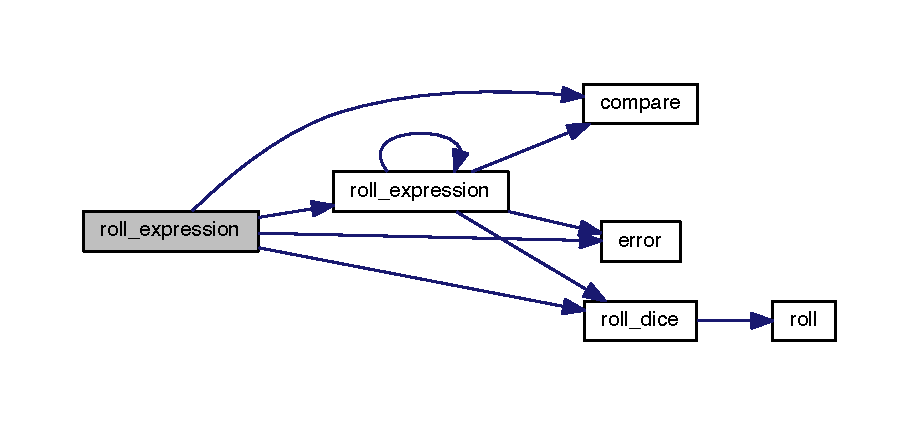
\includegraphics[width=350pt]{roll_8h_ad4c76f688ad79c99d3c39f54358964c8_cgraph}
\end{center}
\end{figure}



%--- End generated contents ---

% Index
\backmatter
\newpage
\phantomsection
\clearemptydoublepage
\addcontentsline{toc}{chapter}{Index}
\printindex

\end{document}
